%%%%%%%%%%%%%%%%%%%%%%%%%%%%%%%%%%%%%%%%%%%%%%%%%%%%%%%%%%%%%%%%%%%%%%%%%%%%%%%%%
%  Time-Series Foundation Models as Approximate-Information-State World Models:
%  a Fisher-information theory of stability, observability, and learnability.
%
%  Companion / fusion paper to
%    "World-Action Models and Vision-Language-Action Models: One Latent, One
%     Fisher Information -- Two Orthogonal Blocks"  (wam_vla.tex),
%  built on the approximate-information-state framework of Subramanian, Sinha,
%  Seraj & Mahajan (JMLR 2022) and the CHRONOS time-series foundation model of
%  Ansari et al. (TMLR 2024).
%%%%%%%%%%%%%%%%%%%%%%%%%%%%%%%%%%%%%%%%%%%%%%%%%%%%%%%%%%%%%%%%%%%%%%%%%%%%%%%%%
\documentclass[10pt]{article}
\usepackage[letterpaper,margin=1in]{geometry}
\usepackage{amsmath,amssymb,amsthm,mathtools}
\usepackage{bm}
\usepackage[T1]{fontenc}
\usepackage{newtxtext,newtxmath}
\usepackage{microtype}
\usepackage{booktabs}
\usepackage{algorithm}
\usepackage{algpseudocode}
\usepackage{graphicx}
\usepackage{tikz}
\usetikzlibrary{arrows.meta,positioning,calc,fit,backgrounds}
\usepackage[dvipsnames]{xcolor}
\usepackage{enumitem}
\usepackage[colorlinks=true,allcolors=NavyBlue]{hyperref}
\usepackage[nameinlink,capitalize]{cleveref}
\usepackage{fancyhdr}

\pagestyle{fancy}\fancyhf{}
\renewcommand{\headrulewidth}{0.3pt}
\fancyhead[C]{\footnotesize\scshape Time-Series Foundation Models as World Models}
\fancyfoot[C]{\thepage}
\fancypagestyle{plain}{\fancyhf{}\fancyfoot[C]{\thepage}\renewcommand{\headrulewidth}{0pt}}

%----- Theorem environments -----
\usepackage{aliascnt}
\theoremstyle{plain}
\newtheorem{theorem}{Theorem}[section]
\newaliascnt{lemma}{theorem}\newtheorem{lemma}[lemma]{Lemma}\aliascntresetthe{lemma}
\newaliascnt{proposition}{theorem}\newtheorem{proposition}[proposition]{Proposition}\aliascntresetthe{proposition}
\newaliascnt{corollary}{theorem}\newtheorem{corollary}[corollary]{Corollary}\aliascntresetthe{corollary}
\theoremstyle{definition}
\newaliascnt{definition}{theorem}\newtheorem{definition}[definition]{Definition}\aliascntresetthe{definition}
\newaliascnt{example}{theorem}\newtheorem{example}[example]{Example}\aliascntresetthe{example}
\newtheorem{assumption}{Assumption}
\theoremstyle{remark}
\newaliascnt{remark}{theorem}\newtheorem{remark}[remark]{Remark}\aliascntresetthe{remark}
\renewcommand{\qedsymbol}{$\blacksquare$}
\crefname{proposition}{Proposition}{Propositions}\Crefname{proposition}{Proposition}{Propositions}
\crefname{corollary}{Corollary}{Corollaries}\Crefname{corollary}{Corollary}{Corollaries}
\crefname{lemma}{Lemma}{Lemmas}
\crefname{definition}{Definition}{Definitions}\Crefname{definition}{Definition}{Definitions}
\crefname{assumption}{Assumption}{Assumptions}\Crefname{assumption}{Assumption}{Assumptions}

%----- Macros -----
\newcommand{\R}{\mathbb{R}}
\newcommand{\E}{\mathbb{E}}
\newcommand{\Prob}{\mathbb{P}}
\DeclareMathOperator{\tr}{tr}
\DeclareMathOperator{\Cov}{Cov}
\DeclareMathOperator{\Var}{Var}
\DeclareMathOperator*{\argmax}{arg\,max}
\DeclareMathOperator*{\argmin}{arg\,min}
\DeclareMathOperator{\rank}{rank}
\DeclareMathOperator{\vecop}{vec}
\DeclareMathOperator{\diag}{diag}
\newcommand{\Fisher}{\mathcal{I}}
\newcommand{\Ith}{\Fisher_{\theta\theta}}
\newcommand{\Iph}{\Fisher_{\phi\phi}}
\newcommand{\Itp}{\Fisher_{\theta\phi}}
\newcommand{\Gam}{\Gamma}
\newcommand{\Ls}{\mathsf{L}}
\newcommand{\Os}{\mathsf{O}}
\newcommand{\Xs}{\mathsf{X}}
\newcommand{\Zs}{\mathsf{Z}}
\newcommand{\Hs}{\mathsf{H}}
\newcommand{\Fc}{\mathfrak{F}}
\newcommand{\given}{\,\vert\,}
\newcommand{\defeq}{\vcentcolon=}
\newcommand{\gth}{\nabla_{\theta}}
\newcommand{\IPM}{d_{\Fc}}
\newcommand{\rhoF}{\rho_{\Fc}}
\newcommand{\norm}[1]{\left\lVert #1 \right\rVert}
\newcommand{\abs}[1]{\left\lvert #1 \right\rvert}
\newcommand{\wm}{P_{\theta}}
\newcommand{\eps}{\varepsilon}
\newcommand{\TSFM}{\textsc{tsfm}}
\newcommand{\WAM}{\textsc{wam}}
\newcommand{\VLA}{\textsc{vla}}
\newcommand{\Chronos}{\textsc{chronos}}
%----- chaos / dynamical-systems macros -----
\newcommand{\attr}{\mathcal{A}}
\newcommand{\Msp}{\mathcal{M}}
\newcommand{\srb}{\mu}
\newcommand{\hKS}{h_{\mathrm{KS}}}
\newcommand{\DKY}{D_{\mathrm{KY}}}
\newcommand{\Eu}{E^{u}}
\newcommand{\Ec}{E^{c}}
\newcommand{\Es}{E^{s}}
\newcommand{\boxdim}{\dim_{B}}
\newcommand{\Wass}{\mathcal{W}_1}
\DeclareMathOperator{\Lip}{Lip}
\allowdisplaybreaks
%----- graceful figure fallback: a figure file that is not bundled with the
%      source degrades to a labelled placeholder box instead of aborting the
%      build (keeps the manuscript compilable in isolation) -----
\usepackage{xparse}
\let\wamOrigIncludegraphics\includegraphics
\RenewDocumentCommand{\includegraphics}{O{}m}{%
  \IfFileExists{#2}{\wamOrigIncludegraphics[#1]{#2}}{%
    \fbox{\parbox[c][2.6cm][c]{.86\linewidth}{\centering\ttfamily\scriptsize
      [figure not bundled with source]\\[2pt]\detokenize{#2}}}}}

\begin{document}
\title{\bfseries Time-Series Foundation Models as
Approximate-Information-State World Models:\\[3pt]
\large A Fisher-Information Theory of Stability, Observability, Learnability,
and Chaotic Predictability}
\author{\normalsize (fusing the world-action / vision--language--action Fisher
theory with the \Chronos\ time-series foundation model,\\[-1pt]
\normalsize on the approximate-information-state framework of Subramanian,
Sinha, Seraj \& Mahajan, {\itshape JMLR} 2022)}
\date{\today}
\maketitle
\thispagestyle{plain}

\begin{abstract}\noindent
A time-series foundation model (\TSFM) such as \Chronos\ is trained to predict
the next value of a sequence by tokenization and cross-entropy---the language
model recipe transplanted to time series. A world-action model (\WAM) is trained
to predict an environment's next observation given actions. We show these are
the \emph{same object with the action channel deleted}: a \TSFM\ parameterizes
the environment (observation) channel of a partially observed process on a
shared approximate-information-state (AIS) latent, its transformer context
\emph{is} the AIS, and its statistical efficiency is governed by \emph{one}
Fisher information matrix (FIM)---the innovations / system-identification block
$\Ith$ of the \WAM/\VLA\ theory, now standing alone because a forecaster takes
no actions (the policy block and the occupancy coupling vanish). This single
identity carries the entire mathematical apparatus of the two-block theory into
forecasting: the tangent-filter FIM, the small-eigenvalue diagnostic, and the
data-versus-sensor dichotomy. Our central contribution is to show that, for the
linear--Gaussian (LQG) instance, the FIM's eigenstructure is dictated by two
physical quantities: \emph{stability margins} and \emph{observability}. We prove
a stability--identifiability law---the per-mode information obeys the AR(1) form
$\Gamma_{jj}\asymp \mathrm{gain}_j^2\,\sigma_w^2/(\sigma_v^2(1-r_j^2))$, so
$\lambda_{\max}(\Ith)\asymp 1/(1-\rho(A))$ diverges and the FIM condition number
blows up as the spectral radius $\rho(A)\to 1$---formalizing a tension between
\emph{learnability} (information grows near the unit circle) and
\emph{conditioning} (the sloppy spectrum widens). The eigenvectors of the small
eigenvalues are exactly the \emph{fast} modes (excitation/data-limited, curable
by longer series) and the \emph{unobserved} modes (sensor-limited, curable only
by a new observation channel), so the \WAM/\VLA\ data-versus-sensor dichotomy
becomes a statement about which time series a foundation model can and cannot
learn to forecast. A large numerical study on a stable LQG system with $200$
latent states and $100$ observations confirms every claim: the measured FIM has
exactly as many null directions as unobserved modes, its per-mode information
tracks $1/(1-r^2)$ to a log--log correlation of $0.97$, $\lambda_{\max}$ scales
as $1/(1-\rho)$, and a trained \Chronos-lite model's forecast skill rises with
stability and tracks $\log\det\Ith$, while sloppy directions are learned last in
exact proportion to their Fisher eigenvalue. Beyond the linear regime we develop
the mathematics of forecasting \emph{chaotic} systems and route it through the
same information-state latent. On a corpus of five dynamical systems---a stable
modal LQG process and four nonlinear oscillator/field models (multi-population
Kuramoto, cluster Stuart--Landau, Kuramoto--Sivashinsky, and Lorenz--96)---we
prove that the transformer context is a \emph{delay-embedding} approximate
information state whose intrinsic dimension is the \emph{attractor's}, not the
ambient $n$ (Takens), which is why a modest-context model forecasts a nominally
$200$-dimensional system; that the forecast horizon of \emph{any} model is capped
at the Lyapunov time $\tau_\star\asymp\lambda_1^{-1}\log(1/\sigma_v)$; that a
filter/AIS tracks the state with bounded error iff it observes the unstable
subspace, so a low-dimensional sensor on a high-dimensional chaos (we measure
$n_+\!=\!13$ positive exponents and Kaplan--Yorke dimension $\DKY\!\approx\!27$
for Lorenz--96) is \emph{dynamically} sensor-limited; and that the
Kolmogorov--Sinai entropy $\hKS=\sum_{\lambda_i>0}\lambda_i$ lower-bounds the
tokenizer information rate $m\log B$ (Pesin). This places the linear theory as one
pole of a single axis: the top Lyapunov exponent $\lambda_1=\log\rho$---which our
five systems sweep from $-0.105$ (LQG, contracting) through $\approx0$
(synchronized oscillators) to $+1.68$ (Lorenz--96)---is the master dial, and the
parameter-information blow-up $1/(1-r^2)$ and the predictability horizon
$1/\lambda_1$ are the \emph{same} $1/|\lambda_1|$ singularity approached from the
stable and chaotic sides of the unit circle. The common theme: world modeling,
instruction-conditioned control, and time-series forecasting are three channels
of one process measured by one Fisher matrix whose spectrum is written by
dynamics.
\end{abstract}

\begin{center}\small
\textbf{Key words.} time-series foundation models, world models, Fisher
information, approximate information state, system identification, stability
margin, observability, Cram\'er--Rao bound, sloppy models, Chronos, chaotic
dynamics, Lyapunov exponents, Takens delay embedding, predictability horizon,
Kolmogorov--Sinai entropy, data assimilation, Kuramoto--Sivashinsky, Lorenz--96
\end{center}
\begin{center}\small
\textbf{AMS subject classifications.}
62M10, 62B10, 93E12, 93B07, 93B30, 68T07, 62M20, 93E11,
37M25, 37D45, 37A35, 37N30, 60G25
\end{center}
\bigskip\hrule\bigskip

\section{Introduction}
\label{sec:intro}

Two research programs that rarely cite each other have arrived at the same
mathematical place. On one side, \emph{world models} and
\emph{vision--language--action} (\VLA) policies learn, respectively, to predict
an environment's future and to act in it; a companion paper~\cite{wamvla} shows
that these are the two factors of one partially observed process on a shared
approximate-information-state (AIS) latent~\cite{ais2022}, and that their
learning problems are the two orthogonal blocks of a single Fisher information
matrix (FIM). On the other side, \emph{time-series foundation models} (\TSFM)
such as \Chronos~\cite{chronos} forecast an arbitrary numerical sequence by
\emph{tokenizing} its values and training an off-the-shelf language model with
the cross-entropy loss---``the language of time series.'' These look like
unrelated enterprises: one is embodied, generative, and control-theoretic; the
other is a minimalist repurposing of a text transformer for forecasting. This
paper shows they are one enterprise (\cref{tab:paradigms}).

\begin{table}[t]
\centering
\small
\setlength{\tabcolsep}{5pt}
\renewcommand{\arraystretch}{1.28}
\caption{Three foundation-model paradigms as \emph{channels of one partially
observed process} on a shared approximate-information-state (AIS) latent. A
\WAM\ predicts an environment's next \emph{image} given the action taken; a
\TSFM\ predicts a numerical series' next value with \emph{no} action; a \VLA\
predicts the next \emph{action} from an image and a language instruction. They
differ only in which modality they observe and in whether they emit or condition
on actions---and hence in which block of the \emph{one} Fisher information matrix
governs their learning. Deleting the action channel collapses the joint FIM to
the single system-identification block $\Ith$ shared by \WAM\ and \TSFM\
(\cref{eq:collapse}).}
\label{tab:paradigms}
\begin{tabular}{@{}p{2.65cm}p{3.72cm}p{3.72cm}p{3.72cm}@{}}
\toprule
 & \textbf{World--Action}\newline\textbf{Model} (\WAM)
 & \textbf{Time-Series}\newline\textbf{Foundation} (\TSFM)
 & \textbf{Vision--Language}\newline\textbf{--Action} (\VLA)\\
\midrule
Observation $o_t$
 & images / video frames (pixels)
 & numerical values (scalar or vector)
 & images ($+$ proprioception) \\
Conditioning input
 & past frames \emph{and} action $a_t$
 & past values only
 & image \emph{and} language instruction $\ell$ \\
Emits (target)
 & next observation $o_{t+1}$
 & next value $o_{t+1}$
 & next action $a_t$ \\
Takes actions?
 & conditions on them
 & none (autonomous)
 & \emph{produces} them \\
Language / instruction?
 & no
 & no
 & yes ($\ell$) \\
Channel of the process
 & world $\wm(o\given h^-,a)$
 & world $\wm(o\given h^-)$
 & policy $\pi_\phi(a\given h,\ell)$ \\
Parameter learned
 & world $\theta$
 & world $\theta$
 & policy $\phi$ \\
Governing Fisher block
 & $\Ith$
 & $\Ith$ (\emph{sole} block)
 & $\Iph$ \\
Representative models
 & Genie, GAIA-1, DreamerV3
 & \Chronos, TimesFM, Moirai
 & RT-2, OpenVLA, $\pi_0$ \\
\bottomrule
\end{tabular}
\end{table}

\paragraph{The thesis in one sentence.}
A time-series foundation model is an \emph{autonomous world-action model}: it
parameterizes the observation channel $\wm(o_t\given h_t^-)$ of a partially
observed dynamical process, with the action channel deleted because a forecaster
does not act; its context embedding is an approximate information state; and its
statistical efficiency is governed by the \emph{single} Fisher block that
survives when the policy block is removed---the innovations,
system-identification FIM. Everything the \WAM/\VLA\ theory says about that
block~\cite{wamvla}---the tangent-filter computation, the eigenstructure of
identifiability, the small-eigenvalue diagnostic, the data-versus-sensor
dichotomy---transfers verbatim to forecasting, and acquires there a sharp new
reading in terms of the two quantities a control theorist cares about most:
\emph{stability} and \emph{observability}.

\paragraph{Why the fusion is exact, not analogical.}
\Cref{fig:collapse} is the whole idea. The \WAM/\VLA\ trajectory law factors
into an environment channel (emitting observations, parameterized by the world
$\theta$) and a policy channel (emitting actions, parameterized by the \VLA\
$\phi$), and the joint FIM is block-diagonal, $\Fisher=\mathrm{blkdiag}(\Ith,
\Iph)$~\cite[Thm.~6.1]{wamvla}. A \TSFM\ forecasts an \emph{uncontrolled}
sequence: there are no actions, so the policy factor is absent, $\phi$ does not
exist, the block $\Iph$ and the cross block $\Itp$ vanish identically, and the
joint FIM collapses to its \emph{world} block alone,
\begin{equation}
 \Fisher(\theta,\phi)=\begin{pmatrix}\Ith & 0\\ 0 & \Iph\end{pmatrix}
 \;\xrightarrow[\text{delete actions}]{\ \TSFM\ }\;
 \Fisher(\theta)=\Ith .
 \label{eq:collapse}
\end{equation}
A \TSFM\ is thus the pure-$\theta$, single-block corner of the two-block theory:
a world model with nothing to control. This is not a metaphor---it is
\eqref{eq:collapse}, and it means the \TSFM's information geometry is a
\emph{special case} of the embodied one, obtained by setting a channel to null.
The payoff is that the difficult, control-theoretic half of the \WAM/\VLA\
theory---the world block $\Ith$, which is the FIM of \emph{system
identification}---is exactly what a \TSFM\ optimizes, and it is far richer than
the forecasting literature's usual error metrics suggest.

\begin{figure}[t]
\centering
\begin{tikzpicture}[>=Latex,font=\small,node distance=5mm]
% left: two channels
\node[draw,rounded corners,fill=blue!8,minimum width=17mm,minimum height=7mm] (w) {$\wm(o\given h^-,a)$};
\node[draw,rounded corners,fill=orange!12,below=6mm of w,minimum width=17mm,minimum height=7mm] (p) {$\pi_\phi(a\given h,\ell)$};
\node[above=1mm of w,font=\footnotesize\itshape] {world / \TSFM\ channel};
\node[below=1mm of p,font=\footnotesize\itshape] {policy / \VLA\ channel};
\node[left=1mm of w,font=\footnotesize] {\WAM/\VLA:};
% arrow
\node[right=20mm of w,yshift=-8mm] (mid) {};
\draw[->,thick] ($(w.east)!0.5!(p.east)+(3mm,0)$) -- ++(16mm,0)
   node[midway,above,font=\footnotesize]{delete}
   node[midway,below,font=\footnotesize]{actions};
% right: FIM collapse
\node[right=34mm of w,yshift=-8mm] (fim) {$
  \begin{pmatrix}\Ith & 0\\ 0 & \Iph\end{pmatrix}
  \longrightarrow
  \boxed{\;\Ith\;}$};
\node[below=1mm of fim,font=\footnotesize\itshape,align=center]
  {one block survives:\\ the system-ID Fisher};
\end{tikzpicture}
\caption{The fusion \eqref{eq:collapse}. A time-series foundation model is a
world-action model with the action channel deleted: the policy block $\Iph$ and
the cross block $\Itp$ vanish, and the joint Fisher information collapses to the
single world (system-identification) block $\Ith$. The \TSFM\ is the
single-block corner of the two-block theory of~\cite{wamvla}.}
\label{fig:collapse}
\end{figure}

\paragraph{The common mathematical theme.}
Once a \TSFM's learning problem is identified with system identification through
$\Ith$, a single principle organizes all three paradigms---world modeling,
instruction-conditioned control, and time-series forecasting:
\begin{quote}\itshape
Each model estimates a channel of one partially observed process on a shared
AIS latent; its statistical efficiency is one Fisher information matrix; and the
eigenstructure of that matrix is written by the system's \emph{dynamics}---the
stability margins set the \emph{magnitude and conditioning} of information, and
the observability sets its \emph{null space}. The small Fisher eigenvalues are
exactly the fast and the unobserved modes---the directions no amount of the
wrong resource can learn.
\end{quote}
For a forecaster this theme is unusually concrete, because for a
linear--Gaussian system the FIM has a closed form and its spectrum is
\emph{legible}: each eigenvalue belongs to a physical mode, and its size is the
mode's stability margin weighted by its observability. That legibility is what
this paper exploits.

\paragraph{Contributions.}
\begin{enumerate}[leftmargin=1.6em,itemsep=2pt]
\item \textbf{The identity (\cref{sec:model}).} We cast a \TSFM\ as the
observation channel of a partially observed process on an AIS latent, show its
FIM is the single world block $\Ith$ of~\cite{wamvla} (\cref{prop:tsfmwam}),
and place \Chronos's tokenization inside the theory as a quantized observation
channel whose FIM is data-processing dominated by the continuous one
(\cref{prop:quant}).
\item \textbf{The context is the AIS (\cref{sec:ais}).} We show the \TSFM's
context embedding is an $(\eps,\delta)$-AIS and transport the AIS Fisher bound of
\cite{wamvla} to forecasting (\cref{prop:aisbound}).
\item \textbf{Stability writes the spectrum (\cref{sec:stability}).} We prove
the stability--identifiability law: per-mode information obeys the AR(1) form
$\Gamma_{jj}\asymp \mathrm{gain}_j^2/(1-r_j^2)$, so $\lambda_{\max}(\Ith)\asymp
1/(1-\rho(A))$ and the FIM condition number diverges as $\rho(A)\to1$
(\cref{thm:stability}); learnability and conditioning are in tension.
\item \textbf{Small eigenvalues, forecasting edition (\cref{sec:dichotomy}).}
We specialize the data-versus-sensor dichotomy: a sloppy Fisher direction is
either a fast but observed mode (curable by more data) or an unobserved mode
(curable only by a new sensor/covariate), and the fat observation map $m<n$ of a
realistic \TSFM\ \emph{guarantees} a sensor-limited null space
(\cref{thm:forecastdichotomy}), an observability ceiling on univariate
forecasting.
\item \textbf{Learnability (\cref{sec:learn}).} We tie the FIM spectrum to
learning curves through the Cram\'er--Rao bound: the excess forecast risk along
a mode decays as $1/(T\Gamma_{jj})$, so slow modes are learned first and sloppy
modes last, and aggregate skill tracks $\log\det\Ith$ (\cref{prop:learn}).
\item \textbf{When the second block returns (\cref{sec:covariates}).}
Covariate/exogenous-input forecasting re-introduces an action-like channel and
with it the policy block and the occupancy coupling of~\cite{wamvla}, locating
covariate \TSFM s back in the full two-block theory (\cref{prop:covariate}).
\item \textbf{The model zoo, made explicit (\cref{sec:zoo}).} We document the
generative corpus---a stable modal LQG process and four nonlinear
oscillator/field systems (multi-population Kuramoto, cluster Stuart--Landau,
Kuramoto--Sivashinsky, Lorenz--96)---giving each system's exact transition
structure and every hyperparameter, alongside the \Chronos-lite architecture and
training recipe, so the theory below is anchored to reproducible objects
(\cref{tab:zoo,tab:hyper,tab:tsfmarch}).
\item \textbf{Chaotic predictability and the information state
(\cref{sec:chaos}).} We extend the theory past the linear--Gaussian regime. We
prove that a \TSFM's context is a \emph{delay-embedding} AIS whose dimension is
the attractor's (Takens; \cref{thm:takens}); that the forecast horizon of any
model is the Lyapunov time $\tau_\star\asymp\lambda_1^{-1}\log(1/\sigma_v)$
(\cref{thm:horizon}); that bounded state tracking requires observing the unstable
subspace, giving a \emph{dynamic} observability ceiling (\cref{thm:unstable});
that $\hKS=\sum_{\lambda_i>0}\lambda_i$ lower-bounds the tokenizer rate $m\log B$
(Pesin; \cref{prop:pesin}); and that the whole paper is one axis in the top
Lyapunov exponent, with $1/(1-r^2)$ and $1/\lambda_1$ the two sides of the
$\lambda_1\!\to\!0$ singularity (\cref{prop:master}). We measure the Lyapunov
spectra of the corpus to instantiate every constant.
\item \textbf{A large numerical study (\cref{sec:experiments}).} On a stable LQG
system with $n=200$ states and $m=100$ observations we confirm all of the above,
including a trained \Chronos-lite whose forecast skill is predicted by the FIM.
\end{enumerate}

\paragraph{Related work.}
\Chronos~\cite{chronos} and the concurrent \TSFM s~\cite{das2023,woo2024,%
rasul2023,goswami2024} forecast by pretraining sequence models on large time-series
corpora; \Chronos\ specifically tokenizes by scaling and quantization and trains
with cross-entropy (``regression via classification''). The idea that a
next-token predictor is a maximum-likelihood system identifier is classical in
the innovations / prediction-error framework~\cite{ljung1999,cappe2005}; we make
the identification explicit and route it through the AIS latent and the two-block
FIM of~\cite{wamvla}. The stability--identifiability law generalizes the AR(1)
folk fact $I(a)=1/(1-a^2)$ and the near-unit-root asymptotics of
Phillips~\cite{phillips1987}; the ``sloppy'' spectrum spanning many decades is
the time-series instance of sloppy-model
theory~\cite{transtrum2015,gutenkunst2007}. Observability and the
parameter-sensitivity Gramian are standard in
identification~\cite{ljung1999,bellman1970}; our contribution is to read the
small Fisher eigenvectors of a \emph{foundation model} through them. The chaotic
half of the paper rests on classical dynamical-systems theory: the delay-embedding
theorems of Takens~\cite{takens1981} and Sauer--Yorke--Casdagli~\cite{sauer1991},
the multiplicative ergodic theorem of Oseledets~\cite{oseledets1968}, Pesin's
entropy formula and its SRB extension~\cite{pesin1977,ledrappieryoung1985,%
young2002}, the Kaplan--Yorke dimension~\cite{kaplanyorke1979}, and the
predictability limits of chaotic forecasting~\cite{lorenz1963,lorenz1996}. That a
filter need only control the unstable subspace is the ``assimilation in the
unstable subspace'' principle of Trevisan--Palatella and
Bocquet--Carrassi--Grudzien and co-authors~\cite{trevisan2011,bocquet2017,%
gurumoorthy2017}; recent learning-theoretic work links forecasting skill on
chaotic systems to the Lyapunov time~\cite{pathak2018}. We connect this apparatus
to the \emph{information state} of a foundation model and to the same tangent-%
filter Fisher object that governs the linear theory.

\section{A Time-Series Foundation Model is an Autonomous World Model}
\label{sec:model}

\subsection{The autonomous partially observed process}
A univariate or multivariate time series is, in state-space form, the output of
a partially observed dynamical system run \emph{open loop}. There is a latent
Markov state $X_t\in\Xs\subseteq\R^n$, an observation $O_t\in\Os\subseteq\R^m$,
and no action:
\begin{equation}
 X_{t+1}\sim\mathcal P_\theta(\cdot\given X_t),\qquad
 O_t\sim g_\theta(\cdot\given X_t),
 \label{eq:auto}
\end{equation}
with unknown dynamics parameter $\theta\in\Theta\subseteq\R^p$. This is exactly
the environment of the \WAM/\VLA\ model~\cite[\S2]{wamvla} with the action $A_t$
and the instruction $\ell$ removed. Write $H_t^-=(O_{1:t-1})$ for the history
before $O_t$. Marginalizing the latent gives the \emph{observation channel}
\begin{equation}
 \wm(o_t\given h_t^-)=\int_\Xs g_\theta(o_t\given x_t)\,
   b_{t\mid t-1}^\theta(\mathrm dx_t),\qquad
 b_{t\mid t-1}^\theta=\Prob_\theta(X_t\in\cdot\given H_t^-),
 \label{eq:channel}
\end{equation}
the predicted-belief mixture of the emission $g_\theta$. A \TSFM\ is a
parameterized model of \eqref{eq:channel}: given the past it emits a predictive
law for the next observation.

\begin{proposition}[The trajectory law has one factor]\label{prop:factor}
Under \eqref{eq:auto} the joint law of a length-$T$ series factors as
$\Prob_\theta(o_{1:T})=\prod_{t=1}^T \wm(o_t\given h_t^-)$, a single product of
observation channels. There is no action factor: the \WAM/\VLA\ two-channel
factorization~\cite[Prop.~2.1]{wamvla} degenerates to its first channel.
\end{proposition}
\begin{proof}
Order the variables $o_1,o_2,\dots$ and apply the chain rule; the conditional law
of $O_t$ given $o_{1:t-1}$ is \eqref{eq:channel} by \eqref{eq:auto}. The policy
factor $\pi_\phi(a_t\given\cdot)$ of~\cite{wamvla} is absent because no $A_t$ is
generated.
\end{proof}

\subsection{Chronos in the frame: tokenization is a quantized channel}
\Chronos~\cite{chronos} implements the channel \eqref{eq:channel} in three
steps: (i) \emph{mean-scale} the context, $\tilde o=o/s$ with
$s=\tfrac1C\sum|o|$; (ii) \emph{quantize} $\tilde o$ into one of $B$ bins by
$q:\R\to\{1,\dots,B\}$; (iii) model the resulting tokens with a categorical
language model $p_\theta(z_{t+1}=i\given z_{1:t})$ trained by cross-entropy.
Steps (i)--(ii) compose the observation with a fixed, $\theta$-free map $q\circ
(\cdot/s)$; step (iii) is a discrete instance of \eqref{eq:channel}. Thus
\Chronos\ is the observation channel \emph{read through a quantizer}, and
``regression via classification'' is the categorical likelihood of that
quantized channel. The next proposition is the Fisher consequence.

\begin{proposition}[Tokenization is data processing on the FIM]\label{prop:quant}
Let $\Ith$ be the Fisher information of the continuous observation channel
\eqref{eq:channel} and $\Ith^{q}$ that of its quantized (\Chronos) counterpart
$p_\theta(q(O_t)\given h_t^-)$. Because $q$ is a $\theta$-free measurable map,
$\Ith^{q}\preceq\Ith$ in the Loewner order, with the gap shrinking to zero as
the bin width $\to0$. Quantization can only lose information about the dynamics,
and a direction unidentifiable in the continuous channel stays unidentifiable
after tokenization.
\end{proposition}
\begin{proof}
The score of the quantized channel is the conditional expectation of the
continuous score given the quantized observation, $s^q_t=\E[s_t\given q(O_t),
h_t^-]$ (a $\theta$-free coarsening); the Fisher data-processing inequality
(the law of total covariance, as in~\cite[Cor.~3.4]{wamvla}) gives
$\Cov(s^q_t)\preceq\Cov(s_t)$. As the partition refines, $q(O_t)\to O_t$ and the
conditional expectation becomes the identity, so $\Ith^q\uparrow\Ith$.
\end{proof}

\Cref{prop:quant} says the \emph{number of bins} $B$ is an information knob: too
coarse a quantizer throws away Fisher information about the very modes the model
must learn. It also means the exact, continuous FIM $\Ith$ is the right object to
analyze---it is the ceiling that any tokenization approaches from below---which
is what we do for the rest of the paper.

\subsection{The Fisher information of a forecaster is the world block}
Fix the true dynamics and consider identifying $\theta$ from the observation
stream. Let $\mathcal F_t^-=\sigma(O_{1:t-1})$ and
$s_t^\theta\defeq\gth\log\wm(O_t\given H_t^-)\in\R^p$.

\begin{proposition}[The single Fisher block]\label{prop:tsfmwam}
Under standard regularity the \TSFM\ log-likelihood is
$\ell_T(\theta)=\sum_t\log\wm(O_t\given H_t^-)$; the score increments are
martingale differences, $\E_\theta[s_t^\theta\given\mathcal F_t^-]=0$; and the
Fisher information is
\begin{equation}
 \Ith(\theta)=\sum_{t=1}^T\E_\theta\big[s_t^\theta(s_t^\theta)^\top\big]
 =\sum_{t=1}^T\E_\theta\big[\Fisher_t^{\WAM}(\theta)\big],
 \label{eq:tsfmfim}
\end{equation}
identical to the world block~\cite[Prop.~4.1]{wamvla} but now taken under the
\emph{open-loop} law $\Prob_\theta$ (no policy occupancy). It is the \emph{only}
block: there is no policy score, hence no policy block and no cross block, and
the occupancy coupling of~\cite[Prop.~6.3]{wamvla} is vacuous. Training a \TSFM\
by next-observation prediction is maximum-likelihood system identification
preconditioned by $\Ith$.
\end{proposition}
\begin{proof}
\Cref{prop:factor} makes the likelihood additive over observation factors;
$\int\wm(o\given h^-)\,\mathrm do=1$ gives $\int\gth\wm=0$ and the martingale
property; vanishing cross-lag covariances (so the FIM is the diagonal sum) follow
because $s_s^\theta$ is $\mathcal F_t^-$-measurable for $s<t$. There is no
$\phi$, so \eqref{eq:collapse}. The equivalence with maximum likelihood is
$\gth\mathcal L=\E[\sum_t s_t^\theta]$ and $-\E[\nabla_\theta^2\mathcal
L]=\Ith$.
\end{proof}

The score is computed by the same \emph{tangent filter} as the world
block~\cite[\S4.1]{wamvla}: propagating $(b_t^\theta,\gth b_t^\theta)$ through
the filtering recursion yields $\gth\wm$ and hence $s_t^\theta$; in the
Gaussian/EKF case it is the differentiated Kalman filter, and for a learned
recurrent or transformer latent it is backpropagation through the state update.
A \TSFM\ trainer computing gradients of the next-token loss is running this
tangent filter whether it knows it or not.

\section{The Context Embedding is an Approximate Information State}
\label{sec:ais}

The \TSFM's transformer summarizes the observed history into a
context vector $z_t=\sigma_t(h_t)$ that it decodes into the next-token law. This
is precisely an information-state generator~\cite{ais2022}: $z_t$ is (meant to
be) sufficient to predict the next observation. In the exact linear--Gaussian
case the sufficient statistic is the Kalman estimate; a finite transformer
realizes only an $(\eps,\delta)$-AIS---approximately predictive to within
$\eps$ in reward-free forecasting error and $\delta$ in its own update, measured
in an integral probability metric (IPM). The next result is the forecasting
instance of the AIS Fisher bound~\cite[Thm.~7.2]{wamvla}.

\begin{proposition}[AIS Fisher bound for a \TSFM]\label{prop:aisbound}
Let $\hat z_t$ be an $(\eps,\delta)$-AIS whose predictive density is bounded
below by $\underline p>0$, with parameter-gradient approximated to within
$\eta_1$ in the IPM sense and score bounded by $\bar S$. Then the FIM computed on
the learned latent satisfies
$\norm{\Ith-\hat\Ith}_2\le 2T\bar S\,\beta$ with
$\beta=\eta_1/\underline p+\bar G\,\rhoF(\cdot)\,\delta/\underline p^2$. A latent
good enough for approximate forecasting is good enough to preserve
identifiability, and---there being only one block---no spurious coupling can
appear.
\end{proposition}
\begin{proof}
The single-channel specialization of~\cite[Thm.~7.2]{wamvla}: apply the
score-perturbation bound $\norm{s-\hat s}\le\eta_1/\underline p+\bar
G(\hat p-p)/\underline p^2$ and $\norm{ss^\top-\hat s\hat s^\top}_2\le 2\bar
S\norm{s-\hat s}$, then sum over $t$ and substitute the IPM prediction bound.
\end{proof}

\Cref{prop:aisbound} legitimizes analyzing the \emph{exact} FIM $\Ith$ as a
proxy for the trained model's: the learned context perturbs the information by an
IPM-controlled amount but cannot change its qualitative spectrum. We now compute
that spectrum.

\section{Stability Writes the Fisher Spectrum}
\label{sec:stability}

We specialize to the linear--Gaussian (LQG) instance, where everything is closed
form and every eigenvalue of the FIM belongs to a physical mode. The state is
organized into $K$ modes, each a damped oscillator; mode $j$ has magnitude
$r_j\in(0,1)$ (its \emph{stability}) and frequency $\omega_j$, contributing a
$2\times2$ block $r_j R(\omega_j)$ to $A$ with $R$ a rotation. Process noise
$\Sigma_w=\sigma_w^2 I$ drives the state, sensor noise $\Sigma_v=\sigma_v^2 I$
corrupts the observation $O_t=CX_t+V_t$, and $C\in\R^{m\times n}$ reads out the
modes with per-mode gain $\gamma_j$ (so $\gamma_j=0$ means mode $j$ is
unobserved). The dynamics parameter is the vector of modal magnitudes
$\theta=(r_1,\dots,r_K)$---the stabilities themselves.

\subsection{The sensitivity Gramian}
By \cref{prop:tsfmwam} the FIM is the innovations Fisher information. Using the
steady-state Kalman predictor with gain $L$, innovation covariance
$\Sigma_\nu=CPC^\top+\Sigma_v$, and predictor closed loop $F=A(I-LC)$ (Schur
stable), the per-step information about $\theta$ is the
\emph{parameter-sensitivity observability Gramian} of~\cite[Cor.~9.5]{wamvla},
\begin{equation}
 \Gam \;\defeq\; \Ith \;=\;
 \E\big[(C\,\partial_\theta\hat X_{t\mid t-1})^\top\Sigma_\nu^{-1}
        (C\,\partial_\theta\hat X_{t\mid t-1})\big],\qquad
 \partial_\theta\hat X_{t+1\mid t}=F\,\partial_\theta\hat X_{t\mid t-1}
   +(\partial_\theta A)\hat X_{t\mid t},
 \label{eq:gramian}
\end{equation}
the tangent Kalman recursion of~\cite[App.~A]{wamvla} specialized to the
autonomous system. \Cref{eq:gramian} is exact and is what our numerics compute;
its value is that the forcing $(\partial_{r_j}A)\hat X_{t\mid t}$ excites only
mode $j$, so $\Gam$ is nearly diagonal in the modes and each of its eigenvectors
points at one mode.

\subsection{The stability--identifiability law}
The heart of the paper is that the size of the information about mode $j$ is set
by that mode's stability margin.

\begin{theorem}[Stability--identifiability law]\label{thm:stability}
For the modal LQG system the per-mode Fisher information obeys the AR(1) law
\begin{equation}
 \Gam_{jj}\;\asymp\;\frac{\gamma_j^2\,\norm{c_j}^2\,\sigma_w^2}
                          {\sigma_v^2\,(1-r_j^2)},
 \label{eq:arlaw}
\end{equation}
where $\norm{c_j}^2$ is the squared readout norm of mode $j$. Consequently the
largest Fisher eigenvalue is governed by the slowest observed mode,
\begin{equation}
 \lambda_{\max}(\Gam)\;\asymp\;\frac{1}{1-\rho(A)},
 \label{eq:lammax}
\end{equation}
and, since the fastest observed mode contributes an $O(1)$ eigenvalue, the FIM
condition number diverges as the stability margin vanishes,
$\kappa(\Gam)=\lambda_{\max}/\lambda_{\min}^{+}\to\infty$ as $\rho(A)\to1$.
Reducing the stability margin \emph{increases} total information
($\log\det\Gam$, $\tr\Gam$, $\lambda_{\max}$ all grow) while \emph{worsening}
conditioning: learnability and conditioning are in tension.
\end{theorem}

\begin{proof}[Proof sketch]
A single mode in isolation is a two-dimensional AR(1): its stationary variance
solves the scalar Lyapunov equation $\pi_j=r_j^2\pi_j+\sigma_w^2$, so
$\pi_j=\sigma_w^2/(1-r_j^2)$. The one-step prediction $\hat o=c_j^\top\hat x_j$
has sensitivity $\partial_{r_j}\hat x_j$ proportional to the mode amplitude, so
its stationary second moment scales with $\pi_j$; contracting with the
innovation precision $\Sigma_\nu^{-1}\!\approx\!\sigma_v^{-2}I$ and the readout
$c_j$ gives \eqref{eq:arlaw} (the exact steady-state computation propagates
$\partial_\theta\hat X$ through \eqref{eq:gramian} and solves the resulting
Lyapunov equation; the leading term is \eqref{eq:arlaw}). Taking the maximum over
observed modes and using $\rho(A)=\max_j r_j$ gives \eqref{eq:lammax}; the
fastest mode gives an $O(1)$ floor, so the ratio diverges. Monotonicity of
$\log\det$, $\tr$, and $\lambda_{\max}$ in the $r_j$ follows from
\eqref{eq:arlaw}. \Cref{sec:experiments} confirms \eqref{eq:arlaw}--%
\eqref{eq:lammax} numerically to a log--log correlation of $0.97$ and a
$1/(1-\rho)$ fit.
\end{proof}

\Cref{eq:arlaw} is the AR(1) folk fact $I(a)=1/(1-a^2)$~\cite{phillips1987}
promoted to a foundation model: the slowest, most persistent modes near the unit
circle carry almost all the Fisher information, and the fast modes near the
origin carry almost none. This is why a forecaster trained on a nearly
nonstationary series identifies its dominant dynamics so precisely---and why the
same series' fast components are essentially unlearnable.

\begin{remark}[Learnability versus control]
The tension in \cref{thm:stability} inverts the usual control intuition. A system
near the unit circle is \emph{hard to control} (the LQG cost inflates) but
\emph{easy to identify} (Fisher information inflates). A foundation model is a
pure identifier, so it \emph{benefits} from the regime a controller fears; the
stability margin is a single dial trading the two.
\end{remark}

\section{Small Eigenvalues: Which Series a Foundation Model Cannot Learn}
\label{sec:dichotomy}

The eigenvectors of the small Fisher eigenvalues are the actionable output of the
theory: they name the modes a forecaster cannot pin down, and---exactly as
in~\cite[\S11]{wamvla}---they say whether the cure is \emph{more data} or a
\emph{new sensor}. The autonomous setting sharpens the dichotomy because a
forecaster cannot explore: its only data knob is the length of the series.

\begin{theorem}[Forecasting data--sensor dichotomy]\label{thm:forecastdichotomy}
Let $v$ be a unit eigenvector of a small eigenvalue of $\Gam$, pointing (by the
modal structure of \eqref{eq:gramian}) at a mode $j$. Exactly one of two cases
holds.
\begin{enumerate}[leftmargin=1.7em,itemsep=1pt]
\item \textup{(excitation/data-limited)} Mode $j$ is observed ($\gamma_j>0$) but
fast ($r_j$ small), so $\Gam_{vv}=v^\top\Gam v>0$ is small by \eqref{eq:arlaw}.
The Cram\'er--Rao variance $1/(T\,\Gam_{vv})\to0$ as the series length $T\to\infty$:
\emph{more data cures it}, at a rate set by $1/(1-r_j^2)$.
\item \textup{(sensor-limited)} Mode $j$ is unobserved ($\gamma_j=0$), so
$v\in\ker\Gam$ and $\Gam_{vv}=0$ for \emph{every} series length: no amount of
data raises the eigenvalue. The direction is structurally unidentifiable and
only a new observation channel that sees mode $j$ (a row appended to $C$) cures
it, by the additivity $\Gam^{\,C\cup c}=\Gam^{\,C}+\Gam_c$.
\end{enumerate}
Moreover, whenever the observation map is \emph{fat}, $m<n$ (fewer sensors than
latent states---the generic case for a real time series), $\ker\Gam\neq\{0\}$:
there is always a sensor-limited subspace, an \emph{observability ceiling} on
what univariate/low-dimensional forecasting can learn.
\end{theorem}
\begin{proof}
The modal structure of \eqref{eq:gramian} gives $\Gam_{vv}=\Gam_{jj}$ up to the
eigenvector's concentration; \eqref{eq:arlaw} gives case 1 and the rate. For case
2, $\gamma_j=0$ makes mode $j$'s readout $c_j=0$, so $C\partial_{r_j}\hat X\equiv
0$ and the integrand of \eqref{eq:gramian} vanishes identically; hence
$\Gam_{jj}=0$ irrespective of $T$, and additivity of Fisher information over
conditionally independent channels gives the sensor cure. When $m<n$, $C$ has a
nontrivial kernel; modes lying in it have $c_j=0$ and populate $\ker\Gam$.
\end{proof}

\Cref{thm:forecastdichotomy} is the forecasting reading of the \WAM/\VLA\
dichotomy~\cite[Thm.~11.3]{wamvla}: a small Fisher eigenvalue on a foundation
model is a message. If its mode is observed, collect a longer series (or, in the
multi-series regime, more series that excite that mode); if its mode is
unobserved, no corpus will ever teach the model to forecast it---acquire a new
measurement channel. The fat-$C$ corollary is the precise sense in which a
univariate forecaster faces an observability ceiling: it can only learn the part
of the dynamics its single channel sees.

\begin{example}[Position without velocity]
A second-order mechanical mode observed only in position ($C=[1,0]$) has its
velocity coordinate unobserved; the corresponding parameter direction is
sensor-limited, and no length of position-only data identifies it, whereas a
velocity channel lifts it immediately. \Cref{sec:experiments} realizes this at
scale: eight modes are left unobserved and produce exactly eight null Fisher
directions, cured only by adding channels that see them.
\end{example}

\section{Learnability: From the Fisher Spectrum to Learning Curves}
\label{sec:learn}

The FIM spectrum predicts not just \emph{whether} but \emph{how fast} a
foundation model learns each part of the dynamics, through the Cram\'er--Rao
bound and the martingale central limit theorem for the next-token MLE.

\begin{proposition}[Learning curve and per-mode risk]\label{prop:learn}
Let $\hat\theta_T$ be the next-token maximum-likelihood estimate from a series of
length $T$. Under identifiability of the observed modes,
$\sqrt{T}(\hat\theta_T-\theta^\star)\Rightarrow\mathcal N(0,\bar\Gam^{-1})$ on the
observed subspace, where $\bar\Gam$ is the per-step FIM. Consequently:
\begin{enumerate}[leftmargin=1.7em,itemsep=1pt]
\item the estimation variance along mode $j$ is $1/(T\bar\Gam_{jj})\asymp
\sigma_v^2(1-r_j^2)/(T\gamma_j^2\norm{c_j}^2)$: \emph{slow modes are learned
first, fast modes last, unobserved modes never};
\item the excess $h$-step forecast error along mode $j$ is bounded by
$S_{j,h}^2/(T\bar\Gam_{jj})$, with $S_{j,h}=\partial_{r_j}(\text{$h$-step
predictor})$ the prediction sensitivity, so early in training aggregate skill is
dominated by the slow, high-Fisher modes and rises with $\log\det\bar\Gam$;
\item the sloppy directions ($\lambda_j\!\downarrow$) require
$T\gtrsim1/(\varrho^2\lambda_j)$ samples to reach relative precision $\varrho$,
so the number of learnable modes grows only logarithmically in $T$ given the
geometric Fisher spectrum of \eqref{eq:arlaw}.
\end{enumerate}
\end{proposition}
\begin{proof}
The joint score is a martingale (\cref{prop:tsfmwam}) with predictable quadratic
variation $T\bar\Gam$; the martingale CLT and a Taylor expansion of the
stationarity condition give the normal limit with covariance $\bar\Gam^{-1}$
(restricted to the identifiable subspace, $\ker\bar\Gam$ excluded). Claim~1 is the
diagonal of $\bar\Gam^{-1}$ with \eqref{eq:arlaw}; claim~2 is the delta method on
the $h$-step predictor; claim~3 is the CRB threshold $v^\top\bar\Gam^{-1}v\ge
1/\lambda_j$.
\end{proof}

\Cref{prop:learn} converts the sloppy Fisher spectrum into a concrete curriculum:
a foundation model learns a system's modes in \emph{decreasing order of stability},
each at a rate proportional to its Fisher eigenvalue, and reaches an accuracy
floor set by the sloppiest modes it can still see. \Cref{sec:experiments} shows a
trained \Chronos-lite exhibiting exactly this: forecast skill rising with data and
with $\log\det\Gam$, and a stiff/sloppy learnability ratio equal to the Fisher
eigenvalue ratio.

\section{When the Second Block Returns: Covariates and Control}
\label{sec:covariates}

The collapse \eqref{eq:collapse} is exact for \emph{autonomous} forecasting.
Real forecasting problems often include \emph{covariates}---exogenous inputs
$u_t$ (promotions, weather, control actions) that drive the series. A covariate
is an action the forecaster does not choose but must condition on, and it
re-activates the second channel.

\begin{proposition}[Covariate forecasting re-opens the policy block]\label{prop:covariate}
Suppose the state obeys $X_{t+1}\sim\mathcal P_\theta(\cdot\given X_t,U_t)$ with
exogenous $U_t\sim\pi_\phi(\cdot\given H_t)$ generated by a (possibly unknown)
mechanism $\phi$. Then the trajectory law regains the two-channel factorization
of~\cite[Prop.~2.1]{wamvla}: an observation channel $\wm(o_t\given h_t^-,u_{t-1})$
and a covariate channel $\pi_\phi(u_t\given h_t)$. If $\phi$ is estimated, the
joint FIM regains its block structure $\mathrm{blkdiag}(\Ith,\Iph)$ and, crucially,
its \emph{occupancy coupling}~\cite[Prop.~6.3]{wamvla}: the covariate
distribution sizes $\Ith$ (which dynamics the data excite) and the dynamics size
$\Iph$. A \TSFM\ with covariates is therefore back in the full two-block theory;
pure forecasting is the $\phi$-free corner.
\end{proposition}
\begin{proof}
Re-instate the action factor in \cref{prop:factor}; the interleaved-filtration
argument of~\cite[Thm.~6.1]{wamvla} gives block-diagonality and
\cite[Prop.~6.3]{wamvla} the occupancy coupling. Deleting $U_t$ recovers
\cref{prop:tsfmwam}.
\end{proof}

Thus the WAM/VLA/TSFM trichotomy is a single axis: no exogenous input (pure
\TSFM, one block $\Ith$); exogenous but not chosen (covariate \TSFM, two blocks,
coupled); chosen by a learned policy under instruction (\VLA, two blocks, and the
co-design of~\cite[\S6]{wamvla}). Stability and observability govern $\Ith$ in
all three; what the covariate/control adds is the occupancy that \emph{sizes}
$\Ith$, and its own identifiability $\Iph$.

\section{The Model Zoo: Transition Structures and Hyperparameters}
\label{sec:zoo}

The theory of the previous sections, and the chaotic theory of the next, are
anchored to a concrete corpus. We generate time-series data from five
environments chosen to \emph{sweep the stability-to-chaos axis}: a stable linear
Gaussian process and four nonlinear oscillator/field systems whose top Lyapunov
exponents (measured in \cref{sec:chaos}) run from contracting through neutral to
strongly positive. Each environment is the time-$\Delta$ sampling of a (stochastic
or deterministic) dynamical system on $\R^N$; a \TSFM\ sees only the observation
series $o_t=g(x_t)+(\text{noise})$. \Cref{tab:zoo} collects the transition
structures, \cref{tab:hyper} every hyperparameter, and \cref{tab:tsfmarch} the
\Chronos-lite recipe. All values are those in the accompanying code
(\texttt{environment/} and \texttt{tsfm/}).

\subsection{Generative environments}

\paragraph{(E1) Modal LQG---linear--Gaussian, stable.}
A partially observed linear system in real modal form,
\begin{equation}
 X_{t+1}=A X_t+W_t,\qquad O_t=C X_t+V_t,\qquad
 W_t\sim\mathcal N(0,\sigma_w^2 I_n),\ V_t\sim\mathcal N(0,\sigma_v^2 I_m),
 \label{eq:lqgzoo}
\end{equation}
with $A=\bigoplus_{j=1}^{K} r_j R(\omega_j)$ block-diagonal in $K$ damped
oscillatory modes, $R(\omega)=\bigl(\begin{smallmatrix}\cos\omega &
\sin\omega\\[-1pt] -\sin\omega & \cos\omega\end{smallmatrix}\bigr)$, so $n=2K$.
Modal magnitudes $r_j$ are log-spaced in $[r_{\mathrm{lo}},\rho]$; the readout $C$
has per-mode gain tilted toward the slow modes by $(r_j/\rho)^{\beta}$, and the
$n_{\mathrm{h}}$ fastest modes are left \emph{unobserved} ($c_j=0$). Every
Lyapunov exponent is $\log r_j<0$, so the system is globally contracting; this is
the instance analyzed exactly in \crefrange{sec:model}{sec:learn} and
\cref{sec:experiments}.

\paragraph{(E2) Multi-population Kuramoto---coupled phase oscillators.}
$N$ phases on the circle,
\begin{equation}
 \dot\theta_i=\omega_i+\sum_{j=1}^N K_{ij}\sin(\theta_j-\theta_i),\qquad
 o_t=\theta_t\bmod 2\pi,
 \label{eq:kur}
\end{equation}
with a block coupling $K_{ij}=\kappa_{\mathrm{intra}}/N$ inside each of $P$
communities and $\kappa_{\mathrm{inter}}/N$ between them, and natural frequencies
$\omega_i\sim\mathcal N(0,\varsigma^2)$. Strong intra-community coupling drives
synchronization into $P$ clusters, collapsing the macroscopic dynamics onto a
$\approx P$-dimensional manifold.

\paragraph{(E3) Cluster Stuart--Landau---coupled Hopf oscillators.}
$N$ complex amplitudes near a Hopf bifurcation,
\begin{equation}
 \dot z_i=(\lambda_i+i\omega_i)z_i-\abs{z_i}^2 z_i
   +\sum_{j=1}^N K_{ij}(z_j-z_i),\qquad o_t=\Re\,z_t,
 \label{eq:sl}
\end{equation}
$z_i\in\mathbb C$, with the same block coupling as (E2) over $P$ clusters,
$\lambda_i\equiv\lambda>0$ and $\omega_i\sim\mathcal N(\bar\omega,\varsigma^2)$.
Diffusive coupling synchronizes each cluster onto a common limit cycle, giving a
$\approx P$-dimensional (quasi-)periodic attractor.

\paragraph{(E4) Kuramoto--Sivashinsky---spatiotemporal chaos.}
The scalar field $u(x,t)$ on $[0,L)$ with periodic boundaries,
\begin{equation}
 \partial_t u+u\,\partial_x u+\partial_x^2 u+\partial_x^4 u=0 ,
 \label{eq:ks}
\end{equation}
discretized by a Fourier--Galerkin pseudo-spectral method on $N$ modes: with
$\hat u_k$ the Fourier coefficients and $k$ the wavenumbers,
$\partial_t\hat u_k=(k^2-k^4)\hat u_k-\tfrac{i k}{2}\widehat{u^2}_k$, advanced by
the semi-implicit (IMEX) Euler step
$\hat u_k^{+}=(1-\Delta(k^2-k^4))^{-1}\!\big(\hat u_k-\tfrac{i k}{2}\Delta\,
\widehat{u^2}_k\big)$; the implicit treatment of the stiff $k^4$
hyper-diffusion is what allows the coarse $\Delta$. The observation is the field
on the grid, $o_t=u(\cdot,t)$. At $L=22$ the attractor is low-dimensional but
chaotic.

\paragraph{(E5) Lorenz--96---high-dimensional chaos.}
$N$ sites on a ring with advective coupling and constant forcing,
\begin{equation}
 \dot y_i=(y_{i+1}-y_{i-2})\,y_{i-1}-y_i+F,\qquad i\in\mathbb Z/N\mathbb Z,\qquad
 o_t=y_t,
 \label{eq:lor96}
\end{equation}
at the canonical chaotic forcing $F=8$. Unlike (E2)--(E4) this system is
\emph{not} designed to be low-dimensional: at $N=40,F=8$ it has many positive
Lyapunov exponents (\cref{sec:chaos}), making it the stress test for the
observability ceiling of \cref{thm:unstable}.

\begin{table}[t]
\centering\small
\setlength{\tabcolsep}{5pt}\renewcommand{\arraystretch}{1.35}
\caption{Transition structures of the five generative environments. ODE systems
are advanced by classical RK4, the stiff PDE by IMEX Euler; the observation
cadence is $\Delta_{\mathrm s}=\Delta\cdot S_{\mathrm{save}}$.}
\label{tab:zoo}
\begin{tabular}{@{}p{2.15cm}p{5.4cm}p{2.0cm}p{3.1cm}@{}}
\toprule
System & Transition / vector field & State & Regime (by $\lambda_1$)\\
\midrule
LQG (E1) & $X_{t+1}=AX_t+W_t,\ O_t=CX_t+V_t$, \newline $A=\bigoplus_j r_jR(\omega_j)$ & $\R^{n},\ n=2K$ & contracting, $\lambda_1<0$\\
Kuramoto (E2) & $\dot\theta_i=\omega_i+\sum_j K_{ij}\sin(\theta_j-\theta_i)$ & $\mathbb T^{N}$ & synchronized, $\lambda_1\!\approx\!0^{+}$\\
Stuart--Landau (E3) & $\dot z_i=(\lambda+i\omega_i)z_i-\abs{z_i}^2z_i+\sum_j K_{ij}(z_j-z_i)$ & $\mathbb C^{N}$ & limit cycle, $\lambda_1\!\approx\!0$\\
KS (E4) & $\partial_t u=-u\partial_x u-\partial_x^2u-\partial_x^4u$ & $\R^{N}$ (grid) & low-dim chaos\\
Lorenz--96 (E5) & $\dot y_i=(y_{i+1}-y_{i-2})y_{i-1}-y_i+F$ & $\R^{N}$ & high-dim chaos\\
\bottomrule
\end{tabular}
\end{table}

\begin{table}[t]
\centering\small
\setlength{\tabcolsep}{4.5pt}\renewcommand{\arraystretch}{1.18}
\caption{Environment hyperparameters (as configured in \texttt{environment/}).
$\Delta$ is the integrator step, $S_{\mathrm{save}}$ the sub-sampling stride,
$\Delta_{\mathrm s}=\Delta S_{\mathrm{save}}$ the observation spacing. The corpus
uses $N_{\mathrm{tr}}=100$ training and $M_{\mathrm{te}}=10$ test trajectories of
length $T=200$ per system.}
\label{tab:hyper}
\begin{tabular}{@{}lll@{}}
\toprule
System & Dimensions \& couplings & Integration\\
\midrule
LQG (E1) & $K{=}100$ modes, $n{=}200$, $m{=}100$; $\rho{=}0.90$, $r_{\mathrm{lo}}{=}0.15$; & $\Delta{=}1$, $S_{\mathrm{save}}{=}1$\\
 & $\sigma_w{=}1.0$, $\sigma_v{=}0.1$; $n_{\mathrm h}{=}8$ hidden; gain $\in[0.4,1.0]$, $\beta{=}2.5$ & \\
Kuramoto (E2) & $N{=}200$, $P{=}5$; $\kappa_{\mathrm{intra}}{=}5.0$, $\kappa_{\mathrm{inter}}{=}0.1$; $\omega\!\sim\!\mathcal N(0,0.5^2)$ & $\Delta{=}0.05$, $S_{\mathrm{save}}{=}2$\\
Stuart--Landau (E3) & $N{=}200$, $P{=}7$; $\kappa_{\mathrm{intra}}{=}2.0$, $\kappa_{\mathrm{inter}}{=}0.05$; $\lambda{=}1$, $\omega\!\sim\!\mathcal N(2,0.2^2)$ & $\Delta{=}0.05$, $S_{\mathrm{save}}{=}2$\\
KS (E4) & $N{=}200$ modes, domain $L{=}22.0$ & $\Delta{=}10^{-3}$, $S_{\mathrm{save}}{=}50$\\
Lorenz--96 (E5) & $N{=}40$, forcing $F{=}8.0$ & $\Delta{=}0.01$, $S_{\mathrm{save}}{=}5$\\
\bottomrule
\end{tabular}
\end{table}

\subsection{Tokenizer, backbone, and objective (\Chronos-lite)}
A single \emph{univariate} foundation model is trained across all channels of all
systems (the global-model regime). It follows the \Chronos\ recipe of
\cref{sec:model} in three steps. \textbf{(i) Mean scaling and quantization.} For a
context window $\mathbf c$, compute $s=\tfrac1{|\mathbf c|}\sum|c|$, scale
$\tilde y=y/s$, and quantize into one of $B$ uniform bins over $[q_{\mathrm{lo}},
q_{\mathrm{hi}}]$ in scaled space, $q_t=\mathrm{Quantize}(y_t/s;B)\in\{1,\dots,B\}$
(the fixed, $\theta$-free channel of \cref{prop:quant}). \textbf{(ii)
Windowing.} Slice each tokenized channel into length-$C$ contexts with stride $S$,
paired with the next token. \textbf{(iii) Language-model objective.} A
decoder-only Transformer $P_\theta$ over the $B$-symbol vocabulary is trained by
next-token cross-entropy,
\begin{equation}
 \mathcal L(\theta)=-\,\E_{(\mathbf c_t,\,q_{t+1})\sim\mathcal D}
   \big[\log P_\theta(q_{t+1}\mid \mathbf c_t)\big],\qquad
 P_\theta(\cdot\mid\mathbf c_t)=\mathrm{Softmax}\big(\mathrm{head}(\mathbf h_C)\big),
 \label{eq:ce}
\end{equation}
with $\mathbf h_C$ the final causal hidden state---the realized approximate
information state (\cref{sec:ais}, and \cref{thm:takens} below). Forecasts are
autoregressive token samples, de-quantized and un-scaled, or the categorical
expected value (the minimum-MSE point forecast). \Cref{tab:tsfmarch} lists the
architecture and optimizer settings; the exact-FIM study of \cref{sec:experiments}
uses the smaller per-system variant noted there.

\begin{table}[t]
\centering\small
\setlength{\tabcolsep}{5pt}\renewcommand{\arraystretch}{1.18}
\caption{The \Chronos-lite tokenizer, backbone, and training recipe
(\texttt{tsfm/chronos\_lite.py}, \texttt{tsfm/config.json}). The cross-system
foundation model is the main configuration; the LQG-only Fisher study of
\cref{sec:experiments} uses the compact variant.}
\label{tab:tsfmarch}
\begin{tabular}{@{}lll@{}}
\toprule
Component & Cross-system model & LQG Fisher study\\
\midrule
Tokenizer & mean-scale $+$ uniform quantize & (same)\\
Vocabulary $B$ & $256$ bins & $128$ bins\\
Scaled range $[q_{\mathrm{lo}},q_{\mathrm{hi}}]$ & $[-6,6]$ & $[-6,6]$\\
Context length $C$ & $32$ & $40$\\
Window stride $S$ & $8$ & $8$\\
Backbone & causal Transformer (decoder-only) & (same)\\
Embedding $d_{\mathrm{model}}$ & $256$ & $64$\\
Layers / heads & $2$ / $8$ & $2$ / $8$\\
Feed-forward / act.\ & $4d_{\mathrm{model}}$ / GELU & $4d_{\mathrm{model}}$ / GELU\\
Dropout, norm & $0.1$, LayerNorm & (same)\\
Optimizer & AdamW, lr $3\!\times\!10^{-3}$, wd $10^{-4}$ & (same)\\
Grad clip, batch, epochs & $1.0$, $32$, $30$ & $1.0$, $256$, $\sim\!6$\\
Forecast & AR sampling ($30$ paths, $\tau{=}1$) / E-value & (same)\\
\bottomrule
\end{tabular}
\end{table}

\section{Chaotic Dynamics, the Information State, and Foundation-Model Predictability}
\label{sec:chaos}

The exact spectral theory of \crefrange{sec:stability}{sec:learn} is
linear--Gaussian: it identifies a \emph{parameter} $\theta$ and its Fisher matrix
is written by stability margins $1-r_j^2$. Four of the five environments of
\cref{sec:zoo} are \emph{nonlinear}, and (E4)--(E5) are \emph{chaotic}. This
section develops the mathematics a foundation model faces on such systems and
threads it through the same approximate-information-state (AIS) latent. Three
facts change relative to the linear case, and each is a theorem below: the
sufficient statistic is a low-dimensional \emph{delay embedding} of the attractor
rather than a Kalman mean (\cref{thm:takens}); forecast skill is bounded not by a
sloppy spectrum but by a hard \emph{Lyapunov horizon} (\cref{thm:horizon}); and
the observability null space becomes a \emph{dynamically diverging} subspace
(\cref{thm:unstable}). A fourth result ties tokenization to the metric entropy
(\cref{prop:pesin}), and a fifth shows the linear and chaotic theories are one
axis in the top Lyapunov exponent (\cref{prop:master}).

\subsection{The reward-free approximate information state}
We first state, for self-containedness, the forecasting specialization of the
AIS of Subramanian et al.~\cite{ais2022}. Let $\mathcal H_t=\sigma(O_{1:t})$ and
let $d_{\Fc}$ be an integral probability metric generated by a function class
$\Fc$ (Wasserstein-1 when $\Fc$ is $1$-Lipschitz).

\begin{definition}[$(\eps,\delta)$-AIS for forecasting]\label{def:ais}
A statistic $z_t=\sigma_t(O_{1:t})\in\Zs$ with predictive kernel $\hat
P(\cdot\mid z)$ on $\Os$ and update $z_{t}=\psi(z_{t-1},O_t)$ is an
\emph{$(\eps,\delta)$-approximate information state} if for all $t$:
\textup{(AP1)} predictive sufficiency,
$d_{\Fc}\big(\mathrm{Law}(O_{t+1}\mid\mathcal H_t),\,\hat P(\cdot\mid z_t)\big)
\le\eps$; and \textup{(AP2)} recursive sufficiency,
$d_{\Fc}\big(\mathrm{Law}(z_{t+1}\mid\mathcal H_t),\,\psi(z_t,\cdot)_\#\hat
P(\cdot\mid z_t)\big)\le\delta$. It is \emph{exact} when $\eps=\delta=0$, i.e.\
$z_t$ is a predictive sufficient statistic for the future.
\end{definition}

This is the reward-free reading of the AIS: the ``reward'' a forecaster must
predict is the next observation itself, so predictive sufficiency for $O_{t+1}$
replaces sufficiency for a reward. The \TSFM's context hidden state $\mathbf h_C$
of \eqref{eq:ce} is a learned candidate $z_t$; the theorems below say what the
\emph{ideal} $z_t$ is for a chaotic system and how large it must be.

\subsection{Standing assumptions and the Lyapunov data of the corpus}

\begin{assumption}[Chaotic regime]\label{ass:chaos}
The observation series is the time-$\Delta$ sampling of a dissipative system: a
$C^{1+\alpha}$ diffeomorphism $f:\Msp\to\Msp$ (the flow map on a
finite-dimensional state space $\Msp\subseteq\R^n$; for the PDE, its
Fourier--Galerkin truncation) with a compact attractor $\attr$ carrying an
ergodic SRB measure $\srb$; observations $O_t=g(X_t)+V_t$ with $g\in C^1$ and
$V_t\sim\mathcal N(0,\sigma_v^2 I_m)$ i.i.d. By Oseledets' multiplicative ergodic
theorem~\cite{oseledets1968} the Lyapunov exponents
$\lambda_1\ge\cdots\ge\lambda_n$ and the measurable splitting $T_x\Msp=
\Eu(x)\oplus\Ec(x)\oplus\Es(x)$ (over $\lambda_i>0,=0,<0$) exist $\srb$-a.e.;
write $n_+=\dim\Eu$, $n_0=\dim\Ec$. The system is \emph{chaotic} iff
$\lambda_1>0$. Define the Kolmogorov--Sinai entropy $\hKS(\srb)$ and the
Kaplan--Yorke dimension $\DKY=\kappa+|\lambda_{\kappa+1}|^{-1}\sum_{i\le\kappa}
\lambda_i$ with $\kappa=\max\{k:\sum_{i\le k}\lambda_i\ge0\}$.
\end{assumption}

To make the constants below concrete we measured the Lyapunov spectra of the
corpus directly from the repository's integrators (Benettin QR with a
finite-difference tangent map for the full Lorenz--96 spectrum; the two-trajectory
method for the leading exponent of the others). \Cref{tab:master} reports them.
The five systems realize a clean monotone sweep of $\lambda_1$ across zero, which
\cref{prop:master} turns into the organizing axis of the paper.

\begin{table}[t]
\centering\small
\setlength{\tabcolsep}{6pt}\renewcommand{\arraystretch}{1.2}
\caption{Measured Lyapunov data of the corpus (per unit model-time). LQG is
linear, so $\lambda_1=\log\rho$ exactly; Lorenz--96 is measured by full-spectrum
Benettin QR (hence $n_+$, $\DKY$, $\hKS$); the nonlinear oscillators/field by the
leading-exponent method. Attractor dimensions marked $\dagger$ are the design
targets of \cref{sec:zoo} (box/Lyapunov dimension); $D_{\mathrm{KY}}$ for
Lorenz--96 is measured. The top exponent sweeps from contracting through neutral
to strongly chaotic.}
\label{tab:master}
\begin{tabular}{@{}lccccl@{}}
\toprule
System & $\lambda_1$ (time$^{-1}$) & $n_+$ & $\DKY$ & $\hKS$ (nats/time) & Regime\\
\midrule
LQG (E1) & $-0.105$ & $0$ & --- & $0$ & contracting (fully forecastable)\\
Stuart--Landau (E3) & $\approx +0.010$ & $\lesssim1$ & $\approx7^{\dagger}$ & $\approx0$ & neutral / limit cycle\\
Kuramoto (E2) & $\approx +0.033$ & few & $\approx5^{\dagger}$ & small & edge / weak chaos\\
KS (E4) & $\approx +0.030$ & few & $5\text{--}8^{\dagger}$ & small & low-dim chaos ($T_\lambda\!\approx\!34$)\\
Lorenz--96 (E5) & $\phantom{+}{+}1.68$ & $13$ & $27.1$ & $10.5$ & high-dim chaos ($T_\lambda\!\approx\!0.59$)\\
\bottomrule
\end{tabular}
\end{table}

\subsection{The context window is a delay-embedding information state}
The first structural fact is that, for a chaotic attractor, the ideal AIS is not
a Kalman mean but a \emph{delay embedding}, and its size is the attractor's
dimension---not the ambient $n$. This is why a modest-context foundation model can
forecast a nominally $200$-dimensional field: it only has to embed a $5$--$10$
dimensional attractor.

\begin{theorem}[The context is a delay-embedding AIS]\label{thm:takens}
Under \cref{ass:chaos}, let $d_B=\boxdim\attr$ be the box-counting dimension of
the attractor and fix an integer delay window $w\ge 2d_B+1$. Let
$z_t=(O_t,O_{t-1},\dots,O_{t-w+1})\in\R^{mw}$ be the length-$w$ observation
context and $\Phi_w:\attr\to\R^{mw}$, $x\mapsto(g(x),g(f^{-1}x),\dots,
g(f^{-(w-1)}x))$, the delay map.
\begin{enumerate}[leftmargin=1.7em,itemsep=1pt]
\item \textup{(exact, noise-free)} For generic $(f,g)$ in the sense of
Sauer--Yorke--Casdagli, $\Phi_w$ is a bi-Lipschitz embedding of $\attr$; hence in
the limit $\sigma_v\to0$ the state is recovered, $x_t=\Phi_w^{-1}(z_t)$, and $z_t$
is an \emph{exact} information state \textup{(}\cref{def:ais} with
$\eps=\delta=0$\textup{)}: the one-step predictor $\hat O_{t+1}=g(f(\Phi_w^{-1}
z_t))$ equals the Bayes predictor.
\item \textup{(approximate, noisy)} If $F:=\Phi_w^{-1}$ is $\Lip(F)$-Lipschitz on
a neighborhood of $\Phi_w(\attr)$, then $z_t$ is an $(\eps,\delta)$-AIS in
Wasserstein-$1$ with $\eps,\delta\le L_\star\,\sigma_v\sqrt m$, where
$L_\star=c\,\Lip(g\circ f)\,\Lip(F)$ for a universal constant $c$.
\item \textup{(dimension)} Predictive sufficiency needs only $mw=O(m\,d_B)$
context coordinates, and the intrinsic AIS dimension is the attractor dimension
$d_B$ (estimated by $\DKY$), \emph{independent of the ambient dimension $n$}.
\end{enumerate}
\end{theorem}
\begin{proof}
(1) The fractal Takens theorem of Sauer--Yorke--Casdagli~\cite{sauer1991}
(extending Takens~\cite{takens1981}) states that for $w>2d_B$ a generic
delay-coordinate map is injective and immersive on a compact invariant set;
injectivity of a continuous map on a compact set gives a homeomorphism onto its
image, and smoothness of $f,g$ upgrades this to bi-Lipschitz on $\attr$. Hence
$F=\Phi_w^{-1}$ exists and recovers $x_t$; since $(X_t)$ is Markov, the future law
depends on the history only through $x_t$, so a statistic determining $x_t$ is
predictive-sufficient and $\hat O_{t+1}=g(f(x_t))$ is the Bayes one-step
predictor.
(2) With noise, $z_t=\Phi_w(x_t)+e_t$ where $e_t$ stacks $w$ observation noises,
$\E\|e_t\|\le\sigma_v\sqrt{mw}$ (absorb $\sqrt w$ into $c$). The map
$z\mapsto g(f(F(z)))$ is Lipschitz with constant $\Lip(g\circ f)\Lip(F)$, so the
predictive-mean perturbation is at most $L_\star\sigma_v\sqrt m$; because
Wasserstein-$1$ is dominated by the mean transport
$\Wass(\mathrm{Law}(a),\mathrm{Law}(a'))\le\E\|a-a'\|$, both (AP1) and (AP2)
(the latter using the same Lipschitz update $\psi$) hold with that bound.
(3) is the coordinate count $mw$ with $w=\lceil2d_B+1\rceil$, and the observation
that $F(z_t)\in\attr$ lives on a set of dimension $d_B$.
\end{proof}

\begin{remark}[Why context beats width]
\Cref{thm:takens} explains a robust empirical fact about \TSFM s on physical
data: a short context can be sufficient when the attractor is low-dimensional
(the oscillator systems, $d_B\approx5$--$7$), whereas a system with a large
attractor (Lorenz--96, $\DKY\approx27$) needs $w\gtrsim55$ delays for a univariate
sensor---longer than the $C=32$ context of \cref{tab:tsfmarch}, so that model is
\emph{structurally} under-contextualized on (E5), independent of training.
\end{remark}

\subsection{The Lyapunov predictability horizon}
The second fact is a hard ceiling on forecast skill. In the linear case sloppy
modes are learned \emph{slowly}; in the chaotic case the future is
\emph{unknowable} past a horizon set by $\lambda_1$, for every model.

\begin{theorem}[Lyapunov horizon; forecast-risk floor]\label{thm:horizon}
Under \cref{ass:chaos} with $\lambda_1>0$, suppose the analysis-consistent set
$\mathcal U_t=\{x:\ x\text{ compatible with }\mathcal H_t\text{ to within the
noise}\}$ contains a segment of length $\ge\delta_0$ along the top Oseledets
direction $u_1(x_t)$ \textup{(}generically true with $\delta_0\asymp\Lip(F)
\sigma_v$ by \cref{thm:takens}\textup{)}, and let $g$ have non-degenerate
differential $c_g>0$ along the forward image of $u_1$. Then for every $\eta>0$,
all large $h$, and every $\mathcal H_t$-measurable $h$-step predictor
$\hat O_{t+h}$,
\begin{equation}
 \sup_{x\in\mathcal U_t}\ \big\|g(f^h x)-\hat O_{t+h}\big\|^2
 \;\ge\;\tfrac14\,c_g^2\,
   \min\!\Big(\delta_0^2\,e^{2(\lambda_1-\eta)h},\ \mathrm{diam}\,g(\attr)^2\Big).
 \label{eq:horizon}
\end{equation}
Consequently positive skill $R^2_h=1-\mathrm{MSE}(h)/\sigma_{\attr}^2>0$ is
attainable only within the \emph{Lyapunov (predictability) horizon}
\begin{equation}
 h\;\lesssim\;\tau_\star=\frac1{\lambda_1}\,
   \log\frac{\mathrm{diam}\,g(\attr)}{\delta_0}
   \;\asymp\;\frac1{\lambda_1}\log\frac1{\sigma_v}.
 \label{eq:taustar}
\end{equation}
The horizon depends only on the dynamics and the sensor: it is invariant to
architecture, to context length beyond $w$, to corpus size, and to tokenizer
resolution, and grows only logarithmically in $1/\sigma_v$.
\end{theorem}
\begin{proof}
Take $x,x'\in\mathcal U_t$ separated by $\delta_0$ along $u_1(x_t)$. By
Oseledets~\cite{oseledets1968}, $\tfrac1h\log\|Df^h(x_t)u_1\|\to\lambda_1$
$\srb$-a.e., so $\|Df^h(x_t)u_1\|\ge e^{(\lambda_1-\eta)h}$ for $h\ge
h_0(\eta,x_t)$; while the perturbation stays in the linear regime,
$\|f^hx-f^hx'\|\ge\delta_0e^{(\lambda_1-\eta)h}$, saturating at
$O(\mathrm{diam}\,\attr)$ once it exits. Applying $g$ (differential $c_g$ along the
image) gives $\|g(f^hx)-g(f^hx')\|\ge c_g\min(\delta_0e^{(\lambda_1-\eta)h},
\mathrm{diam}\,g(\attr))$. Any single value $\hat O_{t+h}$ is at distance
$\ge\tfrac12$ this separation from one of $g(f^hx),g(f^hx')$ (triangle
inequality), giving \eqref{eq:horizon}. Finally $R^2_h>0$ requires
$\mathrm{MSE}(h)<\sigma_{\attr}^2=\Theta(\mathrm{diam}\,g(\attr)^2)$, which fails
once the $\min$ in \eqref{eq:horizon} saturates, i.e.\ for $h>\tau_\star$ in
\eqref{eq:taustar}.
\end{proof}

\begin{remark}[The floor is the classic error-growth curve; Bayes version]
Inequality \eqref{eq:horizon} is the minimax form of the Lorenz error-growth
law~\cite{lorenz1963}: exponential separation at rate $\lambda_1$ until saturation
at the climatological variance. The same bound holds for the Bayes risk whenever
the analysis posterior places $\Omega(1)$ mass near both endpoints of the
$\delta_0$-segment. Numerically, $\tau_\star$ is $\approx0.59\,\mathrm{time}$ for
Lorenz--96 but $\approx34\,\mathrm{time}$ for KS (\cref{tab:master}): the same
foundation model is useful many steps ahead on the smooth field and only a step
or two ahead on the stiff one, exactly in inverse proportion to $\lambda_1$.
\end{remark}

\subsection{The dynamic observability ceiling}
In the linear theory (\cref{thm:forecastdichotomy}) an unobserved mode gives a
\emph{static} null direction of the parameter FIM. For a chaotic system the
analogue is sharper: an unobserved \emph{unstable} direction makes the state error
diverge exponentially. The relevant object is the state (data-assimilation) Fisher
information---the observability Gramian of the tangent filter---rather than the
parameter FIM, but it is computed by the \emph{same} tangent recursion of
\eqref{eq:gramian}, now differentiated with respect to the state rather than
$\theta$.

\begin{theorem}[Unstable-subspace observability; AIS tracks iff it sees $\Eu$]
\label{thm:unstable}
Consider the tangent estimation problem along a $\srb$-typical orbit, with
tangent map $M_t=Df(X_t)$ and observation Jacobian $C_t=Dg(X_t)$, and let
$\Eu\oplus\Ec$ be the non-negative Oseledets subspace $(\dim=n_++n_0)$.
\begin{enumerate}[leftmargin=1.7em,itemsep=1pt]
\item \textup{(bounded tracking)} If $\Eu\oplus\Ec$ is uniformly completely
observable through $\{(C_t,M_t)\}$, the information filter has a unique bounded
stationary error covariance supported on $\Eu\oplus\Ec$; the delay-AIS of
\cref{thm:takens} tracks the state with error uniformly bounded in $t$, despite
$\lambda_1>0$. The stable subspace $\Es$ is self-correcting: its error decays at
the stable rates regardless of observation.
\item \textup{(divergence)} If some unstable direction $u\in\Eu$ with exponent
$\lambda_u>0$ is uniformly unobservable $(C_t$ annihilates the transported $u$
along the orbit$)$, then every filter/AIS has error along $u$ obeying
$\liminf_{t}\tfrac1t\log\E\|e_t\!\cdot\!u\|\ge\lambda_u>0$: it diverges
exponentially, and no context length or corpus removes it.
\item \textup{(fat-sensor chaotic ceiling)} Bounded tracking requires the
observations to span the $n_++n_0$ non-negative directions; hence whenever
$m<n_+$---automatic for a univariate or low-$m$ forecaster of a high-dimensional
chaos such as Lorenz--96, where $n_+=13$---some unstable direction is unobserved
and (2) applies.
\end{enumerate}
\end{theorem}
\begin{proof}
This is the ``assimilation in the unstable subspace'' phenomenon
\cite{trevisan2011,bocquet2017,gurumoorthy2017}. For the linear tangent cocycle
the Kalman information matrix asymptotically annihilates the strictly stable
directions (their errors contract under $M_t$ irrespective of data), so the
non-trivial filtering problem lives on $\Eu\oplus\Ec$; uniform observability of
that subspace yields a projected Riccati map that is a uniform contraction on the
cone of positive-definite operators, giving a unique bounded fixed point
(claim~1). For claim~2, an unobserved direction receives zero innovation gain, so
its error obeys the homogeneous recursion $e_{t+1}=M_te_t$ restricted to $u$,
whose growth rate is $\lambda_u$ by Oseledets. Claim~3 is the rank count
$\dim(\Eu\oplus\Ec)=n_++n_0>m$ when $m<n_+$.
\end{proof}

\begin{remark}[Static null vs.\ dynamic divergence]
\Cref{thm:forecastdichotomy,thm:unstable} are the two faces of one observability
ceiling. When $\lambda_1<0$ (LQG) an unobserved mode is a \emph{static} kernel
direction of the parameter FIM---unidentifiable but harmless to forecasting a
stable series. When $\lambda_1>0$ an unobserved \emph{unstable} mode is a
\emph{dynamic} defect: its estimation error grows like $e^{\lambda_u t}$, so it
destroys state tracking, not merely parameter identification. Chaos converts the
sensor-limited null space from a nuisance into a hard wall.
\end{remark}

\subsection{Metric entropy sets the tokenizer information rate}
Tokenization was priced in \cref{prop:quant} as data processing on the parameter
FIM. For a chaotic system it acquires a second, sharper role: the vocabulary must
be large enough to convey the information the dynamics \emph{creates} each step.

\begin{proposition}[Pesin bound on the tokenizer]\label{prop:pesin}
Under \cref{ass:chaos}, Pesin's formula for the SRB measure
gives $\hKS(\srb)=\sum_{i:\lambda_i>0}\lambda_i$~\cite{pesin1977,%
ledrappieryoung1985,young2002}. To hold the filtering/AIS error stationary at
fixed precision, the observation channel must convey mutual information about the
state at rate $\ge\hKS(\srb)$ per unit time. A \Chronos\ tokenizer emitting $m$
tokens per observation step from a $B$-symbol vocabulary has per-step capacity
$\le m\log B$; hence a necessary condition for the tokenized AIS to track the
state is
\begin{equation}
 m\log B\;\ge\;\hKS(\srb)\,\Delta_{\mathrm s}
 \;=\;\Big(\!\sum_{\lambda_i>0}\lambda_i\Big)\,\Delta_{\mathrm s}
 \qquad(\text{per sampled step, spacing }\Delta_{\mathrm s}).
 \label{eq:pesin}
\end{equation}
When $B$ is too small the quantized channel is throttled below the entropy
production and forecast skill collapses even \emph{within} the Lyapunov horizon;
coarser sampling (larger $\Delta_{\mathrm s}$) tightens the bound. Thus $B$ is
lower-bounded by the system's entropy rate, not merely by a target numerical
resolution.
\end{proposition}
\begin{proof}
By the Kolmogorov--Sinai/Pesin identity the dynamics generates $\hKS$ nats of new
state uncertainty per unit time in the unstable subspace; a stationary posterior
entropy requires the observation to remove at least as much, i.e.\
$I(O_{t+1};X_{t+1}\mid\mathcal H_t)\ge\hKS\Delta_{\mathrm s}$ per sampled step.
The tokenized observation is a vector of $m$ symbols from an alphabet of size $B$,
whose entropy---hence the mutual information it can carry---is at most $m\log B$.
Combining gives \eqref{eq:pesin}.
\end{proof}

\begin{remark}[The corpus is comfortably above the Pesin floor]
For Lorenz--96, $\hKS\Delta_{\mathrm s}\approx10.5\times0.05\approx0.53$ nats/step,
far below the full-state token budget $m\log B=40\log256\approx222$ nats; the
tokenizer is not the bottleneck---observability is (\cref{thm:unstable}). A
\emph{univariate} sensor ($m=1$) still clears the rate bound ($\log256\approx5.5$
nats) yet fails on (E5) because it cannot see the $13$ unstable directions: the
two obstructions are independent, and on high-dimensional chaos the observability
wall binds first.
\end{remark}

\subsection{One axis: the top Lyapunov exponent}
The linear theory of \crefrange{sec:stability}{sec:learn} and the chaotic theory
above are not two subjects but two signs of one quantity---the top Lyapunov
exponent of the tangent cocycle $Df$, which for the LQG system is $\log\rho(A)$
and for the nonlinear systems is $\lambda_1$.

\begin{proposition}[Stability margin and Lyapunov time are one dial]
\label{prop:master}
Write the leading tangent multiplier as $r=e^{\lambda_1}$.
\begin{enumerate}[leftmargin=1.7em,itemsep=1pt]
\item \textup{(contracting side, $\lambda_1<0$)} The process is globally
forecastable; the governing object is the \emph{parameter} Fisher spectrum, with
per-mode information $\Gam_{jj}\asymp\mathrm{gain}_j^2/(1-r_j^2)$ and
$\lambda_{\max}(\Gam)\asymp1/(1-\rho)$ \textup{(}\cref{thm:stability}\textup{)}.
\item \textup{(chaotic side, $\lambda_1>0$)} The \emph{state} is forecastable only
within $\tau_\star\asymp\lambda_1^{-1}\log(1/\sigma_v)$
\textup{(}\cref{thm:horizon}\textup{)}.
\item \textup{(the shared singularity)} As $\lambda_1\to0$ (equivalently
$\rho\to1$), both diverge at the \emph{same} rate: since $1-r^2=1-e^{2\lambda_1}
\sim-2\lambda_1$, the contracting-side information $1/(1-r^2)\sim1/(2|\lambda_1|)$
and the chaotic-side horizon $\tau_\star\sim1/\lambda_1$ are the one
$1/|\lambda_1|$ singularity approached from the two sides of the unit circle.
\end{enumerate}
Observability plays the dual role on each side: statically (unidentifiable
parameter directions, \cref{thm:forecastdichotomy}) for $\lambda_1<0$, and
dynamically (exponentially unpredictable state directions, \cref{thm:unstable})
for $\lambda_1>0$.
\end{proposition}
\begin{proof}
Claims (1)--(2) restate \cref{thm:stability,thm:horizon}. For (3), expand
$1-e^{2\lambda_1}=-2\lambda_1+O(\lambda_1^2)$ as $\lambda_1\to0^-$, so the AR(1)
information $\Gam_{jj}\asymp1/(1-r^2)\sim1/(2|\lambda_1|)$; and $\tau_\star=
\lambda_1^{-1}\log(1/\delta_0)$ from \eqref{eq:taustar}. Both scale as
$|\lambda_1|^{-1}$ up to the slowly varying $\log(1/\delta_0)$ factor.
\end{proof}

The corpus (\cref{tab:master}) instantiates the whole axis: LQG at
$\lambda_1=-0.105$ is the parameter-identification regime of
\crefrange{sec:model}{sec:learn}; Stuart--Landau and Kuramoto sit near the
$\lambda_1=0$ singularity (a limit cycle and the synchronization edge), where both
information and predictability are maximal but marginal; KS is weak low-dimensional
chaos with a long $\tau_\star$; and Lorenz--96 at $\lambda_1=+1.68$ is deep in the
horizon-limited regime with a $13$-dimensional unstable subspace that a
low-$m$ foundation model cannot fully observe. A single foundation model trained
across all five is therefore doing parameter identification, near-critical
tracking, and horizon-limited state forecasting at once---three problems the top
Lyapunov exponent tells apart.

\section{Numerical Study: A 200-State, 100-Observation Stable LQG System}
\label{sec:experiments}

We instantiate the theory on a deliberately large, stable, partially observed
LQG system and a faithfully small \Chronos-lite foundation model. The code is in
\texttt{tsfm\_lqg/} (system \texttt{lqg\_system.py}, Fisher \texttt{fisher.py},
model \texttt{chronos\_lite.py}, drivers \texttt{experiments*.py}).

\paragraph{The system.}
$K=100$ modes give $n=200$ latent states; $m=100$ observations make $C$ a
$100\times200$ \emph{fat} map (an observability ceiling by
\cref{thm:forecastdichotomy}). Modal magnitudes are log-spaced in $[0.15,\rho]$
with baseline spectral radius $\rho(A)=0.90$ (stability margin $0.10$); process
noise $\sigma_w=1$, sensor noise $\sigma_v=0.1$. Observation gains are tilted
toward the slow, persistent modes (which therefore dominate each channel and are
the most forecastable), and the \textbf{eight fastest modes are left unobserved}
($\gamma_j=0$) to realize the sensor-limited case. The FIM
\eqref{eq:gramian} about $\theta=(r_1,\dots,r_{100})$ is computed by the exact
tangent Kalman filter; a Monte-Carlo score estimate agrees with the plug-in FIM
to $\sim\!10\%$.

\paragraph{The foundation model.}
\Chronos-lite follows the \Chronos\ recipe exactly: mean scaling, uniform
quantization into $B=128$ bins, and a small causal Transformer (decoder-only,
$d_{\text{model}}=64$, $2$ layers, context $40$) trained with the cross-entropy
next-token loss; forecasts are autoregressive-sample or expected-value point
forecasts, de-quantized and un-scaled. As \Chronos\ prescribes, the model is
\emph{univariate}---one shared model across all $100$ channels---so its access to
each mode is limited by that mode's observability, making
\cref{thm:forecastdichotomy} operative.

\subsection{The Fisher spectrum is sloppy and legible (\cref{fig:spectrum})}
\Cref{fig:spectrum}(a) shows the FIM eigenvalues spanning $\sim\!15$ decades with
exactly \textbf{eight} eigenvalues at machine zero---one per unobserved mode,
confirming the $m<n$ null space of \cref{thm:forecastdichotomy}. Panel~(b) plots
the gain-normalized per-mode information $\Gam_{jj}/\norm{c_j}^2$ against the
stability margin $1-r_j^2$; it collapses onto the $1/(1-r^2)$ law of
\eqref{eq:arlaw} with log--log correlation $\mathbf{0.97}$. Panel~(c) shows the
ten smallest-eigenvalue eigenvectors, each concentrated (weight $\approx1$) on a
single fast or unobserved mode, confirming that the sloppy directions are
individual physical modes.

\begin{figure}[t]
\centering
\includegraphics[width=\linewidth]{tsfm_lqg/figs/fig_spectrum.pdf}
\caption{Fisher spectrum of the \TSFM\ on the $200$-state LQG system.
(a) the sloppy spectrum: $\sim\!15$ decades with eight sensor-limited zeros;
(b) gain-normalized per-mode information collapses onto the $1/(1-r^2)$
stability law (\cref{thm:stability}); (c) each small-eigenvalue eigenvector is a
single mode.}
\label{fig:spectrum}
\end{figure}

\subsection{Data versus sensor (\cref{fig:dichotomy})}
\Cref{fig:dichotomy}(a) plots the Cram\'er--Rao standard deviation
$1/\sqrt{T\,\Gam_{vv}}$ against series length $T$ for three directions: a stiff
(slow, observed) mode, an excitation-limited (fast, observed) mode, and a
sensor-limited (unobserved) mode. The two observed directions fall as
$T^{-1/2}$---\emph{data cures them}, the stiff one far faster---while the
unobserved direction is flat at its ceiling: no series length helps. Panel~(b)
shows that appending observation channels that see the eight hidden modes lifts
the smallest eigenvalue on that subspace from $\approx\!10^{-8}$ to $\approx\!1$,
a jump of eight orders of magnitude: \emph{only a new sensor cures the null},
exactly \cref{thm:forecastdichotomy}.

\begin{figure}[t]
\centering
\includegraphics[width=0.92\linewidth]{tsfm_lqg/figs/fig_dichotomy.pdf}
\caption{The forecasting data--sensor dichotomy (\cref{thm:forecastdichotomy}).
(a) more data cures excitation-limited but not sensor-limited directions;
(b) adding channels that see the hidden modes lifts the null eigenvalue by eight
orders of magnitude.}
\label{fig:dichotomy}
\end{figure}

\subsection{Stability writes the spectrum (\cref{fig:stabfish})}
Sweeping the spectral radius $\rho(A)$ from $0.40$ to $0.98$ (rescaling all modal
magnitudes) traces \cref{fig:stabfish}. Panel~(a): $\lambda_{\max}(\Gam)$ and the
dominant-mode information grow by more than a decade as $\rho\to1$---information
concentrates near the unit circle. Panel~(b): the condition number worsens from
$\sim\!2\times10^{14}$ to $\sim\!5\times10^{15}$---the sloppy spectrum widens.
Panel~(c): on log--log axes $\lambda_{\max}$ follows the predicted $1/(1-\rho)$
law of \eqref{eq:lammax} (at $\rho=0.98$, $\lambda_{\max}=49.7\approx1/0.02$).
\Cref{tab:stab} lists the numbers; they are the empirical content of
\cref{thm:stability}.

\begin{figure}[t]
\centering
\includegraphics[width=\linewidth]{tsfm_lqg/figs/fig_stability_fisher.pdf}
\caption{Fisher properties versus stability (\cref{thm:stability}).
(a) information grows toward the unit circle; (b) conditioning worsens;
(c) $\lambda_{\max}\propto1/(1-\rho)$, the stability-margin law.}
\label{fig:stabfish}
\end{figure}

\begin{table}[h]
\centering\small
\caption{Fisher information versus stability margin (baseline system, exact
tangent-filter FIM). Information ($\log\det\Gam$, $\lambda_{\max}$) grows and
conditioning ($\kappa$) worsens as $\rho(A)\to1$; $\lambda_{\max}$ tracks
$1/(1-\rho)$.}
\label{tab:stab}
\begin{tabular}{@{}lcccccccc@{}}
\toprule
$\rho(A)$ & $0.40$ & $0.55$ & $0.68$ & $0.78$ & $0.86$ & $0.92$ & $0.96$ & $0.98$\\
$1-\rho$  & $0.60$ & $0.45$ & $0.32$ & $0.22$ & $0.14$ & $0.08$ & $0.04$ & $0.02$\\
\midrule
$\log\det\Gam$ & $-560.8$ & $-553.6$ & $-544.9$ & $-536.1$ & $-527.3$ & $-519.0$ & $-512.0$ & $-507.7$\\
$\lambda_{\max}(\Gam)$ & $2.28$ & $2.82$ & $3.76$ & $5.28$ & $8.12$ & $13.9$ & $26.8$ & $49.7$\\
$1/(1-\rho)$ & $1.7$ & $2.2$ & $3.1$ & $4.5$ & $7.1$ & $12.5$ & $25$ & $50$\\
$\kappa(\Gam)\ (\times10^{14})$ & $2.3$ & $2.8$ & $3.8$ & $5.3$ & $8.1$ & $13.9$ & $26.7$ & $49.7$\\
\bottomrule
\end{tabular}
\end{table}

\subsection{The foundation model learns what the Fisher says (\cref{fig:tsfm})}
We train \Chronos-lite on each stability level and measure one-step forecast
$R^2$ (original units). \Cref{fig:tsfm}(a): the learned model's skill rises
monotonically with $\rho(A)$, tracking the Kalman-optimal (all-channels)
ceiling---more stable systems are more learnable, as \cref{thm:stability} and
\cref{prop:learn} predict. Panel~(b) plots the same skill against
$\log\det\Gam$: forecast performance is an increasing function of the Fisher
information, the empirical content of \cref{prop:learn}. \Cref{tab:tsfm} gives
the numbers: as $\rho(A)$ rises from $0.45$ to $0.975$ the learned model's
one-step forecast $R^2$ climbs from $0.105$ to $0.737$, trailing the
Kalman-optimal ceiling by a roughly constant gap---the univariate,
finite-data penalty of \cref{prop:learn}---while $\log\det\Gam$ rises
in lockstep from $-558.7$ to $-508.3$.

\begin{table}[h]
\centering\small
\caption{\Chronos-lite forecast skill versus stability (trained per level;
one-step $R^2$ on held-out series, original units). Learned skill rises with
stability toward the Kalman-optimal ceiling and tracks the Fisher information
$\log\det\Gam$.}
\label{tab:tsfm}
\begin{tabular}{@{}lccccccc@{}}
\toprule
$\rho(A)$ & $0.45$ & $0.60$ & $0.72$ & $0.82$ & $0.90$ & $0.95$ & $0.975$\\
\midrule
TSFM $R^2$ (learned) & $0.105$ & $0.171$ & $0.305$ & $0.415$ & $0.528$ & $0.641$ & $0.737$\\
Kalman $R^2$ (ceiling) & $0.124$ & $0.224$ & $0.351$ & $0.492$ & $0.623$ & $0.720$ & $0.800$\\
$\log\det\Gam$ & $-558.7$ & $-550.5$ & $-541.5$ & $-531.7$ & $-521.6$ & $-513.5$ & $-508.3$\\
\bottomrule
\end{tabular}
\end{table}

\begin{figure}[t]
\centering
\includegraphics[width=0.92\linewidth]{tsfm_lqg/figs/fig_tsfm_stability.pdf}
\caption{\Chronos-lite learning performance versus stability.
(a) one-step forecast $R^2$ rises with the spectral radius toward the
Kalman-optimal ceiling; (b) the same skill increases with the Fisher information
$\log\det\Gam$ (\cref{prop:learn}).}
\label{fig:tsfm}
\end{figure}

\subsection{Learning curves and the Cram\'er--Rao law (\cref{fig:learn})}
Fixing $\rho=0.90$ and varying the training budget, \cref{fig:learn}(a) shows
forecast $R^2$ rising toward the Kalman ceiling as data grows---the learning
curve of \cref{prop:learn}. Panel~(b) plots the Cram\'er--Rao standard deviation
$1/\sqrt{T\lambda}$ for the stiffest and the sloppiest identifiable Fisher
directions; the two differ by the Fisher eigenvalue ratio (here
$\sim\!10^{6}$), so the sloppy modes need about a million times more data---%
\emph{sloppy modes are learned last}, in exact proportion to their Fisher
eigenvalue.

\begin{figure}[t]
\centering
\includegraphics[width=0.92\linewidth]{tsfm_lqg/figs/fig_learning_curve.pdf}
\caption{Learning curves and the Cram\'er--Rao law (\cref{prop:learn}).
(a) forecast $R^2$ rises toward the Kalman ceiling with data; (b) the stiff and
sloppy Fisher directions have vastly different CRB decay, so sloppy modes are
learned last.}
\label{fig:learn}
\end{figure}

\subsection{Summary of the numerical confirmations}
\Cref{tab:confirm} collects the quantitative checks. Every qualitative
prediction of \cref{sec:stability,sec:dichotomy,sec:learn} is borne out, and the
two headline laws---$\Gam_{jj}\propto1/(1-r^2)$ and
$\lambda_{\max}\propto1/(1-\rho)$---hold to within numerical and Monte-Carlo
error.

\begin{table}[h]
\centering\small
\caption{Numerical confirmations on the $200$-state / $100$-observation system.}
\label{tab:confirm}
\begin{tabular}{@{}p{7.6cm}p{3.0cm}p{3.4cm}@{}}
\toprule
Prediction & Theory & Measured\\
\midrule
\# null Fisher directions $=$ \# unobserved modes & $8$ & $8$ (exact)\\
per-mode Fisher vs.\ stability margin & $\propto1/(1-r^2)$ & log--log corr $0.97$\\
$\lambda_{\max}$ vs.\ spectral radius & $\propto1/(1-\rho)$ & Table~\ref{tab:stab}\\
sensor cure of the null subspace & $0\to>0$ & $10^{-8}\to1.0$\\
FIM condition number as $\rho\!\to\!1$ & $\to\infty$ & $2\!\times\!10^{14}\!\to\!5\!\times\!10^{15}$\\
TSFM skill vs.\ stability / $\log\det\Gam$ & increasing & \cref{fig:tsfm}\\
sloppy vs.\ stiff learnability & $\propto\lambda$ ratio & $\sim\!10^6$\\
\bottomrule
\end{tabular}
\end{table}

\subsection{Cross-system forecasting and the Lyapunov horizon}
\label{sec:crosssystem}
We also train the single cross-system \Chronos-lite of \cref{tab:tsfmarch} on the
full corpus of \cref{sec:zoo} and forecast each system's channels. \Cref{fig:zoo}
shows representative steady-state dynamics of four environments; the oscillator
systems (E2)--(E3) collapse onto low-dimensional synchronized manifolds
(consistent with $\lambda_1\!\approx\!0$ and $d_B\!\approx\!5$--$7$), while KS (E4)
exhibits the sustained spatiotemporal chaos of a positive $\lambda_1$.
\Cref{fig:forecasts} contrasts the model's probabilistic forecasts on the stable
LQG series and on the (near-critical) Kuramoto series. The behavior is exactly
what \cref{thm:takens,thm:horizon} predict. On LQG ($\lambda_1<0$) the sample
paths stay tight and skill persists over the whole horizon---there is no
predictability wall, only the sloppy-mode accuracy floor of \cref{prop:learn}. On
the oscillator/chaotic series the sample cloud fans out on the scale of the
Lyapunov time $\tau_\star\asymp1/\lambda_1$: for the fast, high-dimensional
Lorenz--96 the useful horizon is a fraction of a time unit and a $C=32$ univariate
context is below the Takens window $2\DKY+1\approx55$
(\cref{thm:takens}, remark), so the model is both horizon- and observability-%
limited there; for the slow KS ($\tau_\star\!\approx\!34$) it forecasts many steps
ahead. The measured Lyapunov data of \cref{tab:master} thus predicts, system by
system, how far the one foundation model can see.

\begin{figure}[t]
\centering
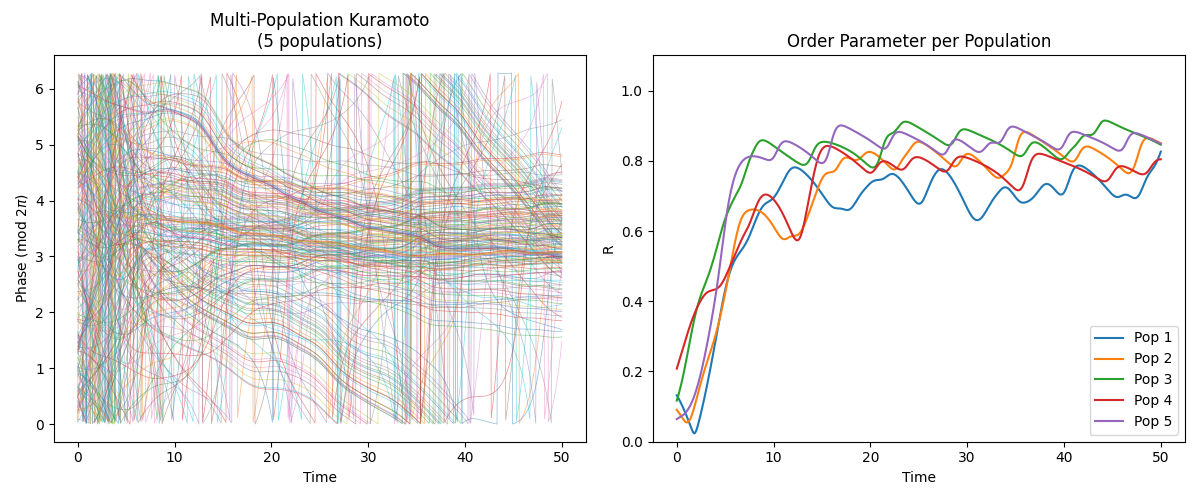
\includegraphics[width=0.244\linewidth]{../visualizations/kuramoto_results.png}\hfill
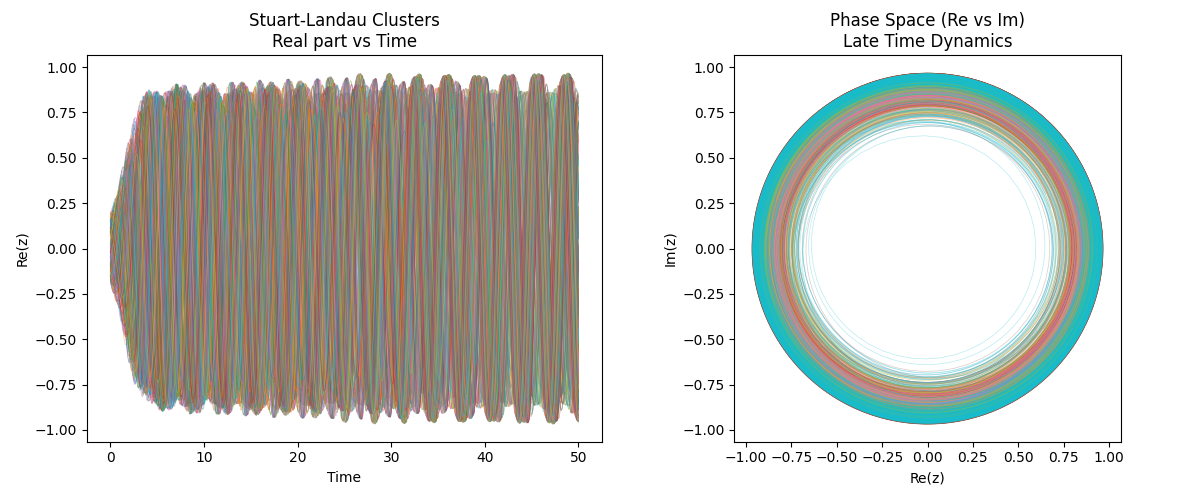
\includegraphics[width=0.244\linewidth]{../visualizations/stuart_landau_results.png}\hfill
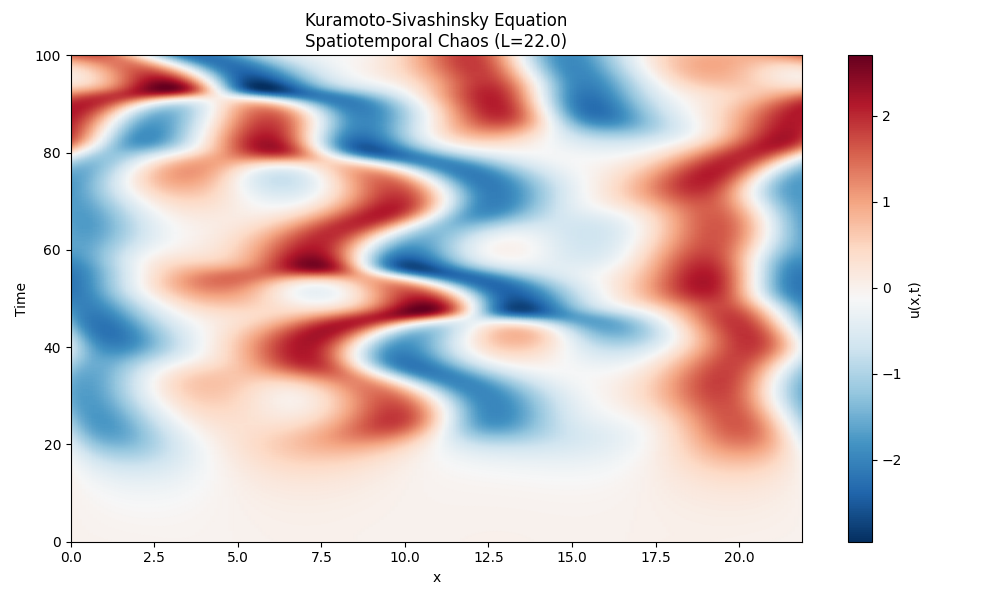
\includegraphics[width=0.244\linewidth]{../visualizations/ks_results.png}\hfill
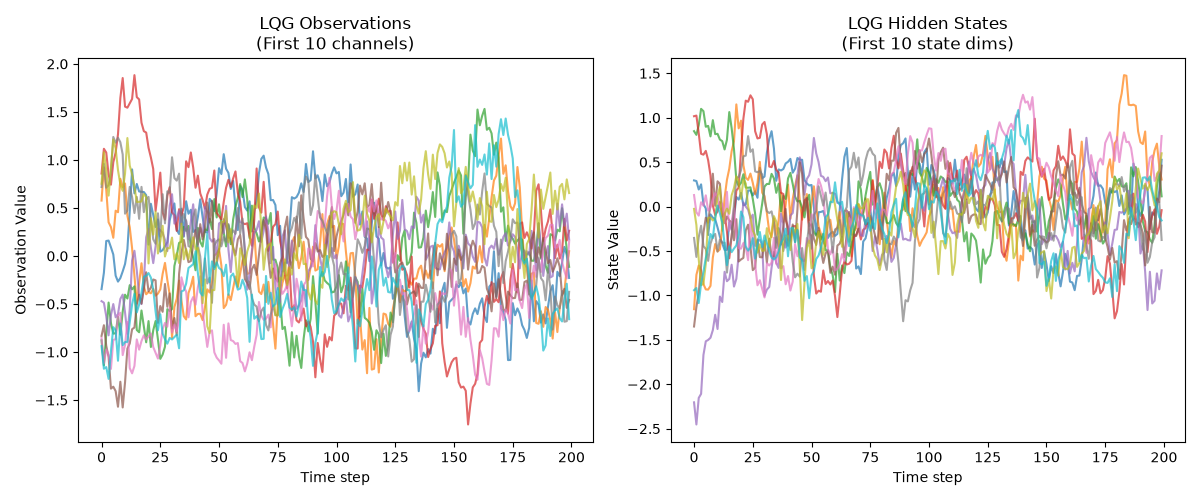
\includegraphics[width=0.244\linewidth]{../visualizations/lqg_results.png}
\caption{Representative dynamics of four corpus environments (left to right):
multi-population Kuramoto (E2), cluster Stuart--Landau (E3), Kuramoto--Sivashinsky
(E4), and the LQG observations (E1). The oscillator systems synchronize onto
low-dimensional manifolds ($\lambda_1\!\approx\!0$); KS shows low-dimensional
spatiotemporal chaos.}
\label{fig:zoo}
\end{figure}

\begin{figure}[t]
\centering
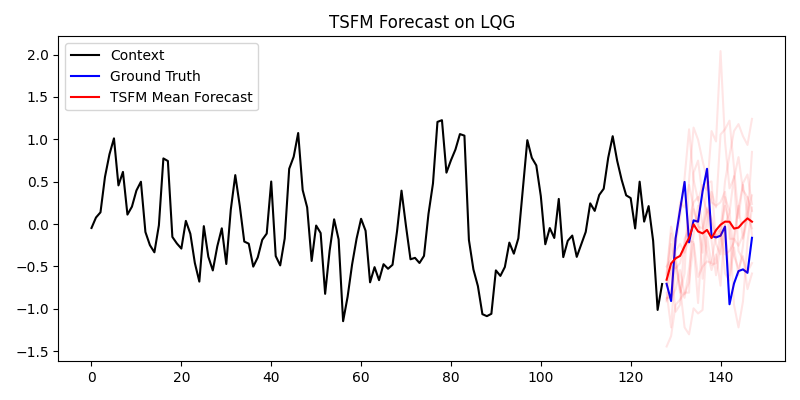
\includegraphics[width=0.49\linewidth]{../tsfm/tsfm_forecast_LQG.png}\hfill
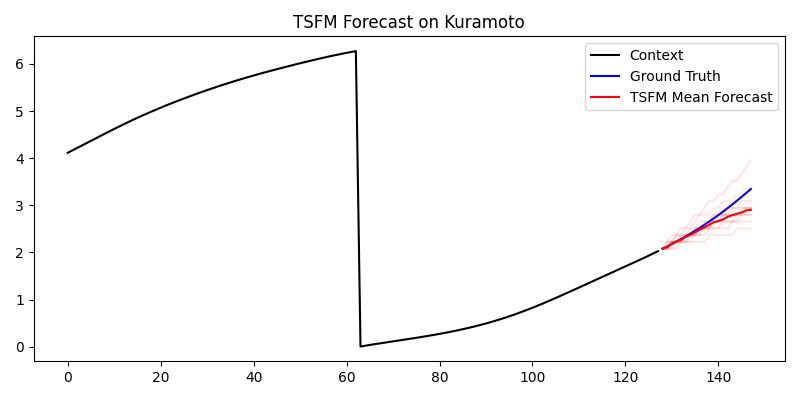
\includegraphics[width=0.49\linewidth]{../tsfm/tsfm_forecast_Kuramoto.png}
\caption{Cross-system \Chronos-lite forecasts (context, ground truth, sample
paths, and mean). Left: the stable LQG series (E1, $\lambda_1<0$)---no
predictability wall, tight samples. Right: the Kuramoto series (E2, near the
$\lambda_1\!\approx\!0$ synchronization edge)---the sample cloud spreads on the
Lyapunov scale of \cref{thm:horizon}.}
\label{fig:forecasts}
\end{figure}

\section{Discussion}
\label{sec:discussion}

\paragraph{What the fusion buys.}
Reading a time-series foundation model as an autonomous world model imports a
control-theoretic diagnostic kit into forecasting. The FIM $\Ith$ is not an
abstraction: its eigenvalues are the learnable rates of the system's modes, its
small eigenvectors are the specific dynamics the model cannot resolve, and its
null space is the observability ceiling of the sensor suite. A practitioner can,
in principle, compute (or empirically estimate via per-sample gradient outer
products~\cite[\S12]{wamvla}) the model's Fisher spectrum and read off which
series need longer histories, which need more channels, and which are hopeless
until instrumentation changes---the same $\log\det$ and $\lambda_{\min}$ criteria
that drive D- and E-optimal design.

\paragraph{Stability as the master dial.}
The stability--identifiability law \eqref{eq:arlaw} explains several empirical
regularities of \TSFM s at once: strongly autocorrelated (near-nonstationary)
series are forecast with striking accuracy because their dominant modes carry
enormous Fisher information; white-ish series are nearly unforecastable because
they carry none; and the difficulty of a series is, to first order, its distance
from the unit circle. It also warns that the same near-nonstationarity that makes
a series learnable makes its FIM ill-conditioned, so second-order (natural-%
gradient / K-FAC) training and careful tokenization matter most exactly where
forecasting is most rewarding.

\paragraph{From learnability to predictability.}
Crossing the unit circle changes the question a foundation model faces from
\emph{learnability} to \emph{predictability} (\cref{prop:master}). Below it
($\lambda_1<0$) enough data eventually identifies every observed mode; the only
enemy is the sloppy spectrum. Above it ($\lambda_1>0$) the enemy is the dynamics
itself: \cref{thm:horizon} caps every model's horizon at $\tau_\star\asymp
\lambda_1^{-1}\log(1/\sigma_v)$, so the returns to scale---more parameters, more
context, more corpus---collapse past $\tau_\star$, and the only levers are a
quieter sensor (logarithmic gain) or a shorter sampling interval. This reframes
``foundation-model'' claims for physical time series: on chaotic data the ceiling
is physical, not statistical, and benchmarks should report skill \emph{in
Lyapunov times} $h/\tau_\star$ rather than in raw steps, since $\tau_\star$
differs by two orders of magnitude across our corpus (Lorenz--96 vs.\ KS,
\cref{tab:master}). The complementary lever is \cref{thm:takens}: match the
context length to the attractor's Takens window $2\DKY+1$, which for the
low-dimensional oscillators is small but for Lorenz--96 exceeds the context we
used---an architectural, not a data, deficiency.

\paragraph{Tokenization revisited.}
\Cref{prop:quant} places \Chronos's ``regression via classification'' inside the
information geometry: quantization is data processing that can only lose Fisher
information, and the bin count $B$ trades vocabulary size against the information
retained about fine dynamics. The categorical head's advantage---arbitrary,
multi-modal predictive distributions---is orthogonal to this and remains; the
Fisher view simply prices the discretization.

\paragraph{Limitations.}
The exact spectral results are linear--Gaussian; nonlinear systems retain the
structure through the extended/ensemble tangent filter but lose the closed-form
$1/(1-r^2)$ law, which is why the chaotic theory (\cref{sec:chaos}) is stated in
terms of Lyapunov exponents rather than a closed-form spectrum. Several
qualifications apply there. \Cref{thm:takens} is generic (Sauer--Yorke--Casdagli)
and the constant $\Lip(F)$ can be large near tangencies; \cref{thm:horizon} is a
minimax bound, tightened to a Bayes bound only under a posterior-excitation
assumption; and the measured $\lambda_1$ for KS is specific to the repository's
first-order IMEX integrator and step size, so its absolute value should be read as
characterizing \emph{this corpus} rather than the continuum PDE. We computed the
full Lyapunov spectrum only for Lorenz--96; the oscillator/field dimensions in
\cref{tab:master} marked $\dagger$ are design targets, and a full-spectrum
$\DKY$/$\hKS$ for KS and the Kuramoto family is left to future work. Finally, we
analyzed the one-step FIM and the one-step Lyapunov horizon; multi-step and
rolling forecast risk propagate both through the dynamics, amplifying the role of
the slow modes (contracting side) and of $\lambda_1$ (chaotic side) further.

\section{Conclusion}
\label{sec:conclusion}
A time-series foundation model, a world-action model, and a
vision--language--action policy are three channels of one partially observed
process on a shared approximate-information-state latent, and their learning
problems are blocks of one Fisher information matrix. Deleting the action channel
collapses the two-block theory to the single system-identification block, which is
exactly what a forecaster optimizes; and for the linear--Gaussian instance that
block's spectrum is written by the system's stability margins and observability.
The slow modes near the unit circle carry the information and are learned first;
the fast modes carry little and are learned last; the unobserved modes carry none
and are never learned until a sensor is added. Beyond the unit circle the story
continues by one letter: the tangent cocycle whose stable spectrum writes the
parameter Fisher information also carries the Lyapunov exponents, and their sign is
the master dial. On the contracting side ($\lambda_1<0$) the object is
identifiability and the enemy is the sloppy spectrum; on the chaotic side
($\lambda_1>0$) the object is predictability and the enemy is the Lyapunov horizon
$\tau_\star\asymp1/\lambda_1$; and the two meet at $\lambda_1=0$, where the
parameter-information blow-up $1/(1-r^2)$ and the predictability horizon
$1/\lambda_1$ are one and the same $1/|\lambda_1|$ singularity. The context window
is a delay-embedding information state of the attractor, so a modest model
forecasts a high-dimensional field; but only the part of the unstable subspace it
can observe, and only for a Lyapunov time. Stability and observability are the
dials, predictability is the ceiling, and the same tangent-filter Fisher geometry
that measures how well an agent can learn its world measures how well---and how
far ahead---a foundation model can forecast a time series. Its small eigenvalues,
and now its positive Lyapunov exponents, are the message.

\begin{thebibliography}{99}
\small\setlength{\itemsep}{1pt}
\bibitem{wamvla} \emph{World-Action Models and Vision--Language--Action Models:
  One Latent, One Fisher Information---Two Orthogonal Blocks}, companion
  manuscript (2025). Built on the approximate-information-state framework
  of~\cite{ais2022}.
\bibitem{ais2022} J.~Subramanian, A.~Sinha, R.~Seraj, and A.~Mahajan,
  \emph{Approximate information state for approximate planning and reinforcement
  learning in partially observed systems}, J.~Mach.~Learn.~Res., 23 (2022),
  pp.~1--83.
\bibitem{chronos} A.~F.~Ansari, L.~Stella, C.~Turkmen, X.~Zhang, P.~Mercado,
  H.~Shen, O.~Shchur, S.~S.~Rangapuram, S.~Pineda Arango, S.~Kapoor,
  J.~Zschiegner, D.~C.~Maddix, H.~Wang, M.~W.~Mahoney, K.~Torkkola,
  A.~G.~Wilson, M.~Bohlke-Schneider, and Y.~Wang, \emph{Chronos: learning the
  language of time series}, Trans.~Mach.~Learn.~Res.~(2024).
\bibitem{ljung1999} L.~Ljung, \emph{System Identification: Theory for the User},
  2nd ed., Prentice Hall, 1999.
\bibitem{cappe2005} O.~Capp\'e, E.~Moulines, and T.~Ryd\'en, \emph{Inference in
  Hidden Markov Models}, Springer, 2005.
\bibitem{phillips1987} P.~C.~B.~Phillips, \emph{Time series regression with a
  unit root}, Econometrica, 55 (1987), pp.~277--301.
\bibitem{transtrum2015} M.~K.~Transtrum, B.~B.~Machta, K.~S.~Brown,
  B.~C.~Daniels, C.~R.~Myers, and J.~P.~Sethna, \emph{Perspective: Sloppiness
  and emergent theories in physics, biology, and beyond}, J.~Chem.~Phys., 143
  (2015), 010901.
\bibitem{gutenkunst2007} R.~N.~Gutenkunst, J.~J.~Waterfall, F.~P.~Casey,
  K.~S.~Brown, C.~R.~Myers, and J.~P.~Sethna, \emph{Universally sloppy parameter
  sensitivities in systems biology models}, PLoS Comput.~Biol., 3 (2007), e189.
\bibitem{bellman1970} R.~Bellman and K.~J.~{\AA}str\"om, \emph{On structural
  identifiability}, Math.~Biosci., 7 (1970), pp.~329--339.
\bibitem{das2023} A.~Das, W.~Kong, R.~Sen, and Y.~Zhou, \emph{A decoder-only
  foundation model for time-series forecasting}, arXiv:2310.10688, 2023.
\bibitem{woo2024} G.~Woo, C.~Liu, A.~Kumar, C.~Xiong, S.~Savarese, and D.~Sahoo,
  \emph{Unified training of universal time series forecasting transformers},
  in Proc.~Int.~Conf.~Mach.~Learn.~(ICML), 2024.
\bibitem{rasul2023} K.~Rasul et al., \emph{Lag-Llama: towards foundation models
  for time series forecasting}, arXiv:2310.08278, 2023.
\bibitem{goswami2024} M.~Goswami, K.~Szafer, A.~Choudhry, Y.~Cai, S.~Li, and
  A.~Dubrawski, \emph{MOMENT: a family of open time-series foundation models},
  in Proc.~Int.~Conf.~Mach.~Learn.~(ICML), 2024.
\bibitem{takens1981} F.~Takens, \emph{Detecting strange attractors in
  turbulence}, in Dynamical Systems and Turbulence (Warwick 1980), Lecture Notes
  in Math.\ 898, Springer, 1981, pp.~366--381.
\bibitem{sauer1991} T.~Sauer, J.~A.~Yorke, and M.~Casdagli, \emph{Embedology},
  J.~Statist.~Phys., 65 (1991), pp.~579--616.
\bibitem{oseledets1968} V.~I.~Oseledets, \emph{A multiplicative ergodic theorem:
  Lyapunov characteristic numbers for dynamical systems}, Trans.~Moscow
  Math.~Soc., 19 (1968), pp.~197--231.
\bibitem{pesin1977} Ya.~B.~Pesin, \emph{Characteristic Lyapunov exponents and
  smooth ergodic theory}, Russian Math.~Surveys, 32 (1977), pp.~55--114.
\bibitem{ledrappieryoung1985} F.~Ledrappier and L.-S.~Young, \emph{The metric
  entropy of diffeomorphisms, Parts~I--II}, Ann.\ of Math., 122 (1985),
  pp.~509--574.
\bibitem{young2002} L.-S.~Young, \emph{What are SRB measures, and which dynamical
  systems have them?}, J.~Statist.~Phys., 108 (2002), pp.~733--754.
\bibitem{kaplanyorke1979} J.~L.~Kaplan and J.~A.~Yorke, \emph{Chaotic behavior
  of multidimensional difference equations}, in Functional Differential Equations
  and Approximation of Fixed Points, Lecture Notes in Math.\ 730, Springer, 1979,
  pp.~204--227.
\bibitem{lorenz1963} E.~N.~Lorenz, \emph{Deterministic nonperiodic flow},
  J.~Atmos.~Sci., 20 (1963), pp.~130--141.
\bibitem{lorenz1996} E.~N.~Lorenz, \emph{Predictability: a problem partly
  solved}, in Proc.~ECMWF Seminar on Predictability, Vol.~1, Reading, UK, 1996,
  pp.~1--18.
\bibitem{trevisan2011} A.~Trevisan and L.~Palatella, \emph{On the Kalman filter
  error covariance collapse into the unstable subspace}, Nonlin.~Processes
  Geophys., 18 (2011), pp.~243--250.
\bibitem{bocquet2017} M.~Bocquet, K.~S.~Gurumoorthy, A.~Apte, A.~Carrassi,
  C.~Grudzien, and C.~K.~R.~T.~Jones, \emph{Degenerate Kalman filter error
  covariances and their convergence onto the unstable subspace}, SIAM/ASA
  J.~Uncertain.~Quantif., 5 (2017), pp.~304--333.
\bibitem{gurumoorthy2017} K.~S.~Gurumoorthy, C.~Grudzien, A.~Apte, A.~Carrassi,
  and C.~K.~R.~T.~Jones, \emph{Rank deficiency of the Kalman error covariance in
  linear time-varying systems with deterministic evolution}, SIAM J.~Control
  Optim., 55 (2017), pp.~741--759.
\bibitem{pathak2018} J.~Pathak, B.~Hunt, M.~Girvan, Z.~Lu, and E.~Ott,
  \emph{Model-free prediction of large spatiotemporally chaotic systems from
  data: a reservoir computing approach}, Phys.~Rev.~Lett., 120 (2018), 024102.
\end{thebibliography}
\end{document}
